\documentclass[12pt]{scrreprt}

%% Allgemeine Hinweise
% 
% - Windows ben�tigt Pearl zum Kompilieren
% - Guter Editor "TexStudio"
% - Nicht vergessen jedes Tex Dokument auf ISO-8859-1 zu stellen
% - Kompilierreihenfolge:
%		1. Makeglossaries
%		2. Biber
%		3. PdfLaTeX
%		4. Interner PDF-Betrachter

%--------------------------------------------------------------------------
% LaTeX packages
%--------------------------------------------------------------------------
\usepackage[ngerman]{babel}		% Neue Deute Rechtschreibung
\usepackage{pdfpages}	% PDF Import
\usepackage{geometry}	% Seitenformatierung (links, rechts usw..)
\usepackage{url}	% Urls
\usepackage{ae}		% Bessere Fonts unterst�tzung
\usepackage[latin1]{inputenc}	% Lateinisch und wichtig f�r MAC
\usepackage[T1]{fontenc}	% Westeurop�ische Kodierung
\usepackage{lmodern}	% Neue deutsche Trennungsregeln, etc 
\usepackage{mathptmx}	% Schriftart (Times New Roman)
\usepackage{acronym}	% Acronyme
\usepackage[onehalfspacing]{setspace}	% Eineinhalb Zeilen Abstand
\usepackage{titlesec}	% Titel Formatierung
\usepackage{hyperref}	% Klickbare Links
\usepackage{minitoc}	% Mini Inhaltsverzeichnis nach jeder �berschrift
\usepackage[headsepline,footsepline]{scrpage2}	% Kopf und Fu�zeilen (Seitenzahl)
\usepackage{listings}	% Quellcode
\usepackage{color}	% Farben f�rs Listing
\usepackage{float}	% Bilder zentrieren
\usepackage[right]{eurosym}
\usepackage[most]{tcolorbox} % Definitionen
\usepackage[autostyle, german=quotes]{csquotes}
\usepackage[backend=biber, style=alphabetic, citestyle=alphabetic]{biblatex}
\usepackage{chngcntr}
\usepackage{caption}
\usepackage{amsmath}
\usepackage{cleveref} % Definitionen
\usepackage[nonumberlist,	% Keine Seitenzahlen anzeigen
						acronym,	% Ein Abk�rzungsverzeichnis erstellen
						toc,	% Eintr�ge im Inhaltsverzeichnis
						section]	% Im Inhaltsverzeichnis auf section-Ebene erscheinen
						{glossaries}	% Glossar

%-----------------------------------------------------------------------------
% Settings
% ********
% Anmerkung: Die meisten Kommandos wurden in der 07_Settings/Settings.tex
% 						Datei erstellt und sollten auch nur dort ver�ndert werden.
%
%-----------------------------------------------------------------------------
% !TEX root = Settings.tex

%################################################################## COMMANDS
%##################################################################
%################################################################## 

\newcommand{\backsl}{\verb|\|} % Backslash

\newcommand{\secline}{\vspace{-1.2em}	% Linie
	\par\noindent\rule{\textwidth}{0.4pt}} 

\newcommand{\emptysite}{\newpage	% Leere Seite
	\thispagestyle{empty}
	\section*{}}

% Glossarzusatz
\renewcommand{\glossarysection}[2][]{\chapter*{#1}}	

% Farbiger Punkt
\newcommand{\tikzcircle}[2][red,fill=red]{\tikz[baseline=-0.5ex]\draw[#1,radius=#2] (0,0) circle ;}

% Abbildungsverzeichnis
\newcommand{\abbildungsverzeichnis}{\newpage
	\phantomsection
	\addstarredchapter{\textbf{Abbildungsverzeichnis}}
	\listoffigures
}

% Tabellenverzeichnis
\newcommand{\tabellenverzeichnis}{\newpage
	\phantomsection
	\addstarredchapter{\textbf{Tabellenverzeichnis}}
	\listoftables
}

% Acronyme
\newcommand{\abkuerzungen}{
	% !TEX root = Acronym.tex
\newpage
\phantomsection
\addstarredchapter{\textbf{Abk�rzungsverzeichnis}}

\chapter*{\huge\textbf{Abk�rzungsverzeichnis}}
\begin{acronym}[Bash]
	\acro{BDD}{Behavior Driven Development}
	\acro{GUI}{Graphical User Interface}
	\acro{HTML}{Hypertext Markup Language}
	\acro{IDE}{Integrated Development Environment}
	\acro{QA}{Quality Assurance}
	\acro{QM}{Qualit�tsmanagement}	
\end{acronym}
}

% Glossar
\newcommand{\glossar}{
	\newpage
	\phantomsection	
	\addstarredchapter{\textbf{Glossar}} % F�gt "Glossar" zum Inhaltsverzeichnis hinzu		
	%\addcontentsline{toc}{chapter}{\textbf{Glossar}}	% F�gt "Glossar" zum Inhaltsverzeichnis hinzu
	\printglossary[style=altlist,title=Glossar]		% Glossar
	\newpage
}

% Heading Style setzen
\newcommand{\headstyle}{
	\pagestyle{scrheadings}	% Style
	\clearscrheadfoot
	\ofoot[\pagemark]{\pagemark}
	\ohead{\headmark}
	\automark[]{chapter}
	\setheadsepline{1pt}
	\setfootsepline{0pt}
}

% Heading Style setzen (Seitenzahl Rechts)
\newcommand{\headstyleright}{
	\pagestyle{scrheadings}	% Style
	\cfoot[]{}	% [plain-Seiten]{normale Seiten} 
	\ofoot[\pagemark]{\pagemark}	% Seitenzahl
	\setheadsepline{0pt}
	\setfootsepline{0pt}
}

\newcommand{\inhaltsverzeichnis}{
	\cleardoublepage\pdfbookmark{\contentsname}{toc}
	\tableofcontents
	\clearpage
	\newpage
}

\newcommand{\literaturverzeichnis}{
	\phantomsection
	\addcontentsline{toc}{chapter}{Literatur}	% �berschrift
	\printbibliography	
}

\newcommand{\anhangstart}{
	\newpage
	%\pagenumbering{arabic}	% Arabische Ziffern
	
	\renewcommand\appendix{\par 
		\setcounter{section}{0}% 
		\setcounter{subsection}{0}% 
		\setcounter{figure}{0}% 
		
		\renewcommand\thesection{\Alph{section}}% 
		\renewcommand\thefigure{\Alph{section}\arabic{figure}}} 
	
	\numberwithin{table}{section} 
	\numberwithin{figure}{section} 
	
	
	\appendix 
	\pagestyle{empty}
	\captionsetup{listof=false}
}

\newcommand{\roemischenummerierung}{
	\pagenumbering{Roman}
}

\newcommand{\arabischenummerierung}{
	\pagenumbering{arabic}
}

%################################################################## OTHER
%##################################################################
%################################################################## 

\titleformat{name=\chapter,numberless}[display]{\normalfont\huge\bfseries}{\titlerule}{-6,9ex}{}[\vspace{3ex}]
\titlespacing{name=\chapter,numberless}{0em}{1.0em}{0em}
\titleformat{\chapter}{\normalfont\huge\bfseries}{\thechapter}{18pt}{\Huge}[{\vspace{0,6ex}\titlerule[0.8pt]\vspace{3ex}}]
\titlespacing{\chapter}{0em}{-4.0em}{0em} % {left}{before}{after}[right]
\titleformat{\section}{\normalfont\LARGE\bfseries}{\thesection}{16pt}{\LARGE}
\titleformat{\subsection}{\normalfont\Large\bfseries}{\thesubsection}{14pt}{\Large}
\titleformat{\subsubsection}{\normalfont\large\bfseries}{\thesubsubsection}{14pt}{\large}

\addbibresource{04_Literatur/Literatur.bib}
\AtBeginDocument{\counterwithin{lstlisting}{section}}
\geometry{a4paper, left=30mm, right=25mm, bottom=25mm, top=25mm}	% Text Formatierung
% !TEX root = Glossar.tex
\makeglossaries

\newglossaryentry{venturecapital}{ 
	name=Venture-Capital, 
	description={ 
		Unter Venture Capital versteht man die Finanzierung eines nicht b�rsennotierten Unternehmens mit Eigenkapital. Dabei wird das Unternehmen in der Regel zum Zeitpunkt der Beteiligung privat gehalten. Entscheidend ist, dass das Eigentum am Unternehmen w�hrend der meisten Zeit der Beteiligung in privaten H�nden liegt \autocite{venture_capital}} 
}

\newglossaryentry{servantleader}{ 
	name=Servant Leader, 
	description={ 
		Ein Servant Leader liebt Menschen und m�chte ihnen helfen. Die Aufgabe eines Servant Leaders ist es daher, die Bed�rfnisse anderer zu ermitteln und zu versuchen, diese Bed�rfnisse zu befriedigen \autocite{servant_leadership}} 
} 

\newglossaryentry{iteration}{ 
	name=Iteration, 
	description={ 
		Eine Iteration ist eine wiederholte Durchf�hrung eines Vorgangs. Die Anzahl der Durchf�hrungen (Iterationen) steht entweder vorher fest oder richtet sich nach der Erf�llung eines Abbruchkriteriums \autocite{definition_iteration} 
	}
} 

\newglossaryentry{stakeholder}{ 
	name=Stakeholder, 
	description={ 
		Anspruchsgruppen sind alle internen und externen Personengruppen, die von den unternehmerischen T�tigkeiten gegenw�rtig oder in Zukunft direkt oder indirekt betroffen sind. Gem�� Stakeholder-Ansatz wird ihnen - zus�tzlich zu den Eigent�mern (Shareholders) - das Recht zugesprochen, ihre Interessen gegen�ber der Unternehmung geltend zu machen \autocite{definition_stakeholder}
	}
}

\newglossaryentry{trialanderror}{ 
	name=Trial and Error, 
	description={ 
		Trial and Error beschreibt einen Weg, ein Ziel zu erreichen oder ein Problem zu l�sen, indem verschiedene Methoden ausprobiert und aus Fehlern gelernt wird \autocite{definition_trialanderror}
	}
}

\newglossaryentry{governance}{ 
	name=Governance, 
	description={ 
		Die Art und Weise, wie in einem Land die Angelegenheiten der Allgemeinheit verwaltet und geregelt werden. \enquote{Governance} ist nicht \enquote{Government} gleich \enquote{Regierung}, sondern umfassender und offener \autocite{definition_governance}
	}
}

\newglossaryentry{workaround}{ 
	name=Workaround, 
	description={ 
		Ein workaround beschreibt eine M�glichkeit, ein Problem zu l�sen, oder etwas trotz des Problems zum laufen zu bekommen, ohne es vollst�ndig zu l�sen \autocite{definition_workaround}
	}
}

\newglossaryentry{coredeliverable}{ 
	name=Core Deliverable, 
	description={ 
		Ein Core Deliverable ist das zentrale Produkt oder Dienstleistung, welches einem Kunden zu Verf�gung gestellt wird \autocite{definition_deliverable}
	}
}

\newglossaryentry{cicd}{ 
	name=Continous Integration, 
	description={ 
		Continous Integration beschreibt einen Softwareentwicklungsprozess, bei dem Teammitglieder h�ufig ihre Arbeit integrieren. Bei jeder Integration wird der Stand automatisch �berpr�ft, um Integrationsfehler so schnell wie m�glich zu erkennen \autocite{definition_ci}
	}
}

\newglossaryentry{devops}{ 
	name=DevOps, 
	description={ 
		Der Begriff besteht aus Development (Dev), der den Softwareentwickler beschreibt, und Operations (Ops), was den IT-Betrieb darstellt. Aus der Kombination beider soll ein Prozessverbesserungsansatz f�r die Bereiche Softwareentwicklung und Systemadministration entstehen. Es wird eine effektivere und effizientere Zusammenarbeit der verschiedenen Bereiche angestrebt \autocite{definition_devops}
	}
}
	% Glossar IMPORT
\setlength{\parindent}{0pt}	% Keine Einr�ckung am Anfang eines Absatzes
\setcounter{biburllcpenalty}{7000}
\setcounter{biburlucpenalty}{8000}

%################################################################## LISTINGS
%##################################################################
%################################################################## 

\renewcommand{\lstlistingname}{Codebeispiel}% Listing -> Codebeispiel
\renewcommand{\lstlistlistingname}{Codeverzeichnis}% List of Listings -> Codeverzeichnis

% Default fixed font does not support bold face
\DeclareFixedFont{\ttb}{T1}{txtt}{bx}{n}{12} % for bold
\DeclareFixedFont{\ttm}{T1}{txtt}{m}{n}{12}  % for normal

% Custom colors
\definecolor{deepblue}{rgb}{0,0,0.5}
\definecolor{deepred}{rgb}{0.6,0,0}
\definecolor{deepgreen}{rgb}{0,0.5,0}
\definecolor{superlightgray}{rgb}{0.97,0.97,0.97}

% Java Style
\lstdefinestyle{java}{
	language=Java,
	basicstyle=\ttm,
	otherkeywords={this},
	breaklines=true,
	tabsize=2,
	keywordstyle=\ttb\color{deepblue},
	emph={MyClass,__init__},          % Custom highlighting
	emphstyle=\ttb\color{deepred},    % Custom highlighting style
	stringstyle=\color{deepgreen},
	frame=tb,                         % Any extra options here
	belowskip=3em,
	belowcaptionskip=1em,
	aboveskip=2em,
	abovecaptionskip=1em,
	captionpos=b,
	showstringspaces=false 
}

% Java Script Style
\lstdefinestyle{travis}{
	language=bash,
	numbers=left,
	stepnumber=5,
	firstnumber=1,
	tabsize=2,
	basicstyle=\ttm,
	breaklines=true,
	alsoletter={:},
	keywords={language:, node_js:, cache:, install:, before_script:, script:},
	keywordstyle=\ttb\color{orange},
	emph={MyClass,__init__},          % Custom highlighting
	emphstyle=\ttb\color{deepred},    % Custom highlighting style
	stringstyle=\color{deepgreen},
	frame=single,                         % Any extra options here
	backgroundcolor=\color{superlightgray},
	ndkeywords={directories:},
	ndkeywordstyle=\ttb\color{deepblue},
	belowskip=2em,
	aboveskip=2em,
	abovecaptionskip=1em,
	captionpos=b,
	showstringspaces=false 
}

% Java Script Style
\lstdefinestyle{cypress}{
	language=Java,
	numbers=left,
	stepnumber=5,
	firstnumber=1,
	tabsize=2,
	basicstyle=\ttm,
	breaklines=true,
	keywords={describe, before, beforeEach, context, it, expect, equal, cy, def},
	keywordstyle=\ttb\color{orange},
	emph={MyClass,__init__},          % Custom highlighting
	emphstyle=\ttb\color{deepred},    % Custom highlighting style
	stringstyle=\color{deepgreen},
	frame=single,                         % Any extra options here
	backgroundcolor=\color{superlightgray},
	ndkeywords={assert, break, case, catch, continue, debugger, default, delete, do, else, false, finally, for, function, if, in, instanceof, new, null, return, switch, this, throw, true, try, typeof, var, void, while, with},
	ndkeywordstyle=\ttb\color{deepblue},
	belowskip=2em,
	aboveskip=2em,
	abovecaptionskip=1em,
	captionpos=b,
	showstringspaces=false 
}

% Python Style
\lstdefinestyle{python}{
	language=python,
	numbers=left,
	basicstyle=\ttm,
	otherkeywords={self},
	keywordstyle=\ttb\color{deepblue},
	emph={MyClass,__init__},          % Custom highlighting
	emphstyle=\ttb\color{deepred},    % Custom highlighting style
	stringstyle=\color{deepgreen},
	frame=tb,                         % Any extra options here
	belowskip=3em,
	aboveskip=2em,
	abovecaptionskip=1em,
	captionpos=b,
	showstringspaces=false  
}

% Bash Style
\lstdefinestyle{bash}{
	language=bash,
	basicstyle=\ttm,
	numbers=left,
	stepnumber=5,
	firstnumber=1,
	backgroundcolor=\color{superlightgray},
	otherkeywords={},
	keywordstyle=\ttb\color{deepblue},
	emph={\$},          % Custom highlighting
	emphstyle=\ttb\color{deepred},    % Custom highlighting style
	stringstyle=\color{deepgreen},
	frame=single,                         % Any extra options here
	showstringspaces=false,
	belowskip=2em,
	aboveskip=2em,
	abovecaptionskip=1em,
	captionpos=b
}

%################################################################## DEFINITONS
%##################################################################
%################################################################## 

\newtcbtheorem[number within=chapter]{Definition}{}{
	enhanced,
	attach boxed title to top left={
		xshift=-1mm,
		yshift=-5mm,
		yshifttext=-1mm
	},
	breakable,
	top=0.5em,
	bottom=-0.5em,
	colback=white,
	colframe=black,
	fonttitle=\bfseries,
	boxed title style={
		size=small,
		colback=black,
		colframe=black,
	} 
}{def}

\newenvironment{definition}[2]{ \begin{Definition}[adjusted title=#1]{}{#2} 
		\textbf{} }{\end{Definition}}

%-----------------------------------------------------------------------------
% START OF DOCUMENT														---------------------
%-----------------------------------------------------------------------------
\begin{document}

% Deckblatt & Einverst�ndnisserkl�rung

\includepdf[pages={1}]{03_PDFs/Deckblatt.pdf}
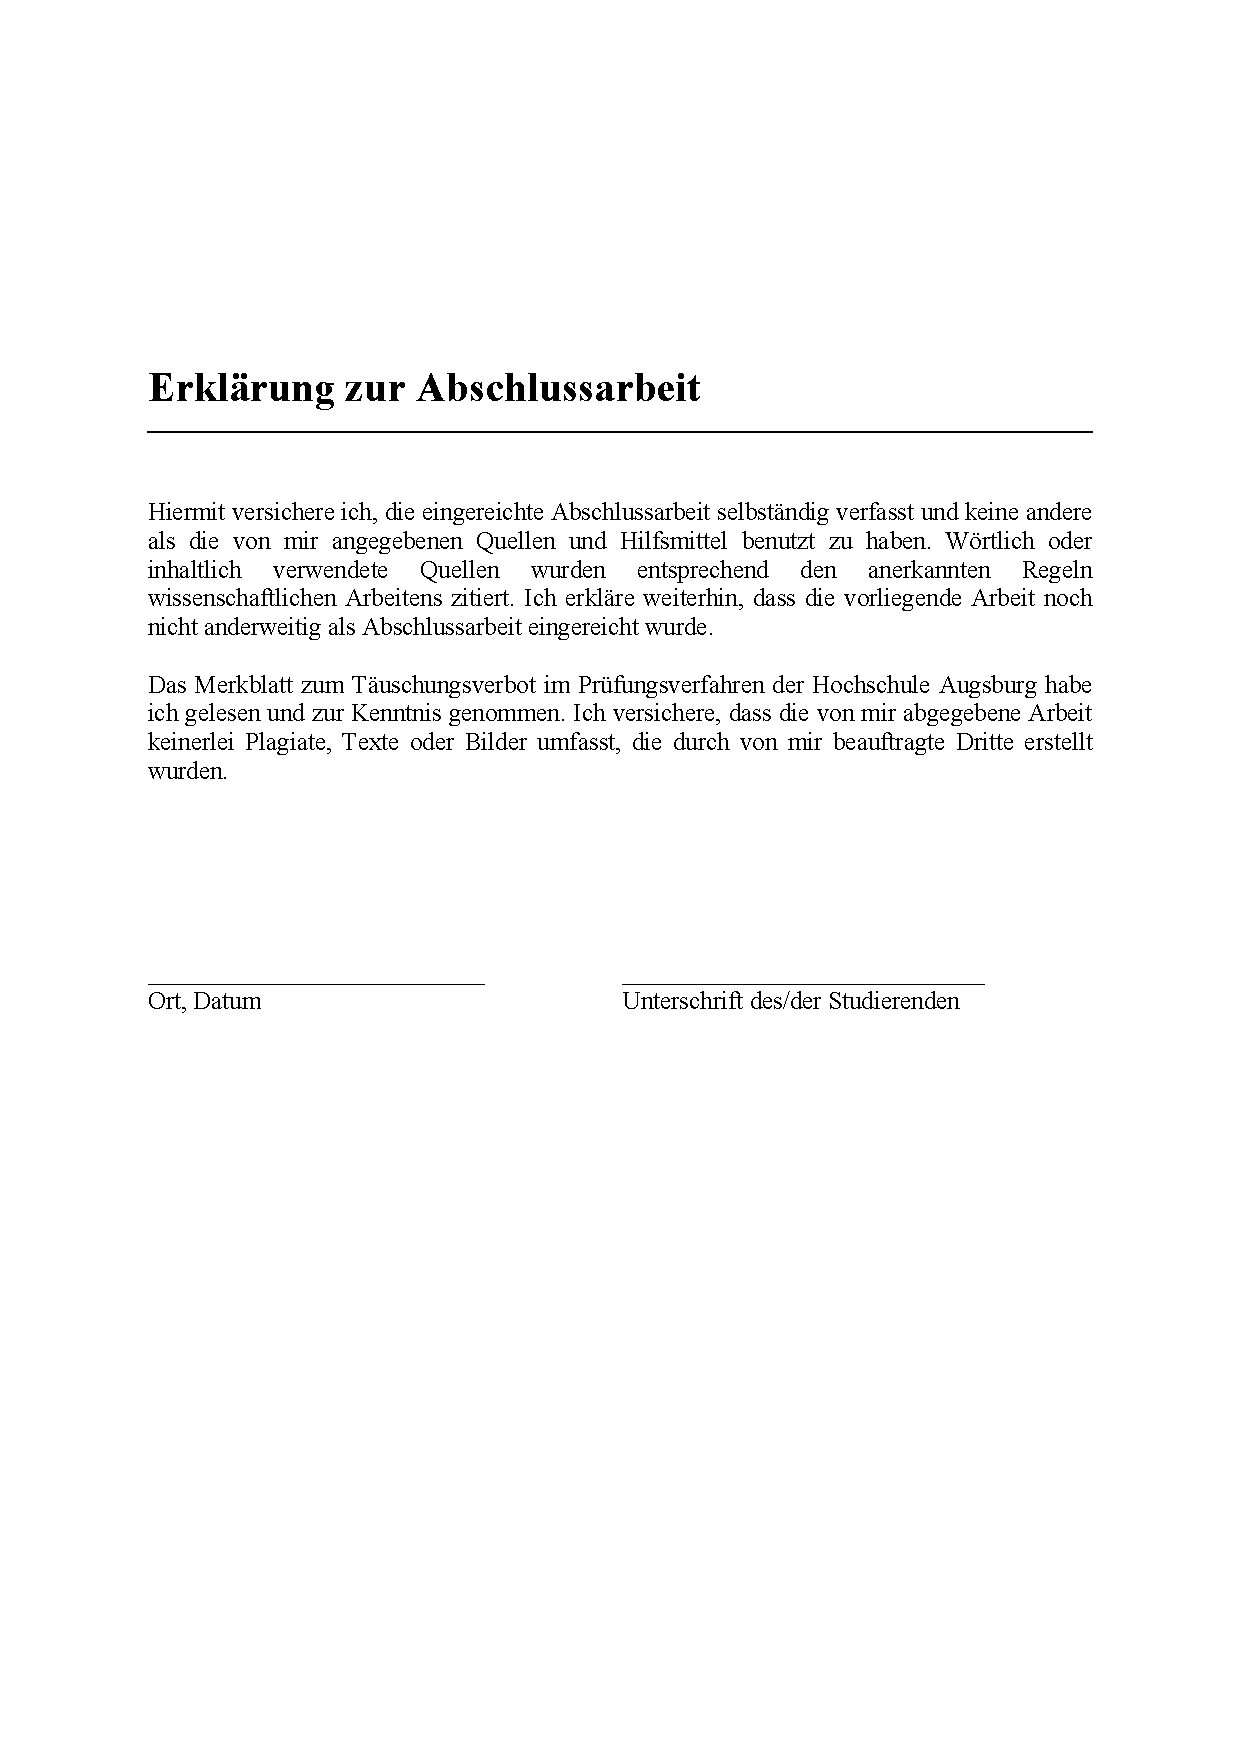
\includepdf[]{03_PDFs/Erstellungserklaerung.pdf}

% Seitenzahlformatierung (rechts)
\headstyleright

% R�mische Ziffern
\roemischenummerierung

% Setze Seitenzahl
\setcounter{page}{3}	

% Danksagung
% !TEX root = Danksagung.tex

\section*{\huge\textbf{Danksagung}}
\secline
\\\\
HIER DANKSAGUNG

\newpage


% Kurzfassung
% !TEX root = Kurzfassung.tex

\section*{\huge\textbf{Kurzfassung}}
\secline
\\\\
Viele Unternehmen sind derzeit im Umbruch in Richtung Agilit�t, obwohl diese oft die Bedeutung noch nicht genau verstehen. Agilit�t wird von einigen geliebt, von anderen nicht verstanden und vom Rest kategorisch abgelehnt. Eine Studie hat gezeigt, dass agiles Arbeiten nicht nur das Teamklima verbessert, sondern Mitarbeiter auch visions-, aufgabenorientierter und innovationsfreudiger arbeiten. Ziel dieser Arbeit ist es, herauszufinden, was genau Unternehmen davon abh�lt, von einer klassischen auf eine agile Arbeitsweise umzusteigen. Um spezifischere Ergebnisse zu erhalten, wurden diese in die drei Arten, Start-up, Mittelstand und Konzern aufgeteilt. Anschlie�end wurde ein Fragebogen erarbeitet, der das Ziel hat, Herausforderungen und Metadaten f�r die jeweiligen Unternehmensarten zu ermitteln. Neben den Ergebnissen der Frageb�gen wurden mithilfe von Erfahrungsberichten und Interviews weitere Daten erhoben. Um aus den Daten, relevante Informationen herauszufiltern, wurde die qualitative Inhaltsanalyse nach Mayring angewendet. Diese hat 45 Herausforderungen und einige Metadaten zutage gebracht. Alle Herausforderungen wurden anschlie�end aus der Sicht jeder Unternehmensart mithilfe der Metadaten bewertet. Die Bewertung hat gezeigt, dass die gr��ten Herausforderungen f�r Start-ups in der Abh�ngigkeit zu den Investoren liegen. Der Mittelstand im Vergleich ist h�ufig traditionell gepr�gt, was Herausforderungen in der Unternehmenskultur und der Verkn�pfung von IT-Systemen mit sich bringt. Dagegen liegen die Herausforderungen von Konzernen, verursacht durch die oft durchwachsene Unternehmensstruktur, oft in der Komplexit�t, der Dauer der Transformation und der damit einhergehenden hohen Kosten. Trotz der Herausforderungen muss jedes Unternehmen f�r sich entscheiden, ob es den langen Weg einer Transformation gehen m�chte. 

\newpage


% Inhaltsverzeichnis
\inhaltsverzeichnis

% Kopf und Fu�zeile
\headstyle

% Abbildungsverzeichnis
\abbildungsverzeichnis

% Tabellenverzeichnis
\tabellenverzeichnis

% Acronyme
\abkuerzungen

% Glossar
\glossar

% Arabische Ziffern
\arabischenummerierung


%-----------------------------------------------------------------------------
% HAUPTARBEIT																	HAUPTARBEIT
%-----------------------------------------------------------------------------
% !TEX root = Einleitung.tex

\chapter{Einleitung}

Jedes Projekt mit dem Ziel Software zu entwickeln, ist individuell. Aus diesem Grund gibt es in den seltensten F�llen wiederholbare Prozesse. Reproduzierbare Prozesse k�nnen durch klare Anweisungen mithilfe anschlie�ender Kontrolle befehligt oder gesteuert werden. Kreative Prozesse hingegen scheitern bei diesem Ansatz, da diese individuell, je nach Situation gesteuert werden m�ssen \autocite[vgl.][]{agiles_projektmanagement}. Um genau diese Art von Steuerung erreichen zu k�nnen, versuchen immer mehr Unternehmen einen agilen Ansatz. Diese Vorgehensweise hat das Ziel, eine kreative Probleml�sung im Team zu f�rdern, da sich Kreativit�t nicht einfach anordnen l�sst \autocite[vgl.][S.VII]{agiler_fuehren}.
\\
\begin{definition}{Definition Agile F�hrung (Quelle: \autocite{agiler_fuehren})}{def:agile_fuehrung}
	\\ 
	Agile F�hrung unterst�tzt Mitarbeiter dabei, schnell und kreativ auf wechselnde Bed�rfnisse von Kunden und M�rkten zu reagieren. Sie ist ein Mindset, eine Haltung. Sie nutzt eine offene Toolbox mit Coachingwerkzeugen, die die Zusammenarbeit verbessern, sowie Methoden zur Reduktion von Komplexit�t.
	\\
\end{definition}

Unternehmens- und F�hrungskulturen sind derzeit in vielen Unternehmen im Umbruch in Richtung Agilit�t. Bei all den Ver�nderungen in diese Richtung wissen viele Unternehmen noch nicht, was es genau bedeutet, als Unternehmen, Team oder F�hrungskraft agiler zu werden. Eine Studie (siehe \autocite[vgl.][VII]{agiler_fuehren}) mit dem Namen \enquote{Teamklima f�r Innovation} wollte herausfinden, ob sich das Teamklima in nicht-agilen Gruppen von den agilen unterscheidet. Das Ergebnis hat gezeigt, dass nicht nur das Teamklima innerhalb agil arbeitender Teams besser war, sondern diese auch visions-, aufgabenorientierter und innovationsfreudiger agieren. Zudem verbessern agile Elemente wie Visualisierung, Teamentscheidung, Retrospektive, iterative Planung und Stand-up-Meetings die Zusammenarbeit \autocite[vgl.][S.VII-VIII]{agiler_fuehren}.
\\\\ 
Das Wort \enquote{Agil} ist eine Art Reizwort, das von einigen geliebt, von anderen nicht verstanden und vom Rest kategorisch abgelehnt wird. So schrieb die amerikanische Zeitschrift \enquote{Forbes!} (siehe \autocite{managers_hate_agile}), dass Manager \enquote{agile} (Agilit�t) hassen. Die Begr�ndung der Zeitschrift f�r die Abwehrhaltung der Manager lag in einem m�glichen Machtverlust, da Agilit�t im Management gerne mit dem Abbau von F�hrung verwechselt wird. Dabei geht es gar nicht um den strikten Abbau von F�hrung, sondern eher um das F�rdern von flacheren Hierarchien. H�ufig wird die Agilit�t abgelehnt, ohne genau zu wissen, was sich dahinter verbirgt. Diejenigen, die nur eine grobe Idee davon haben, begr�nden ihre ablehnende Haltung mit dem Argument, \enquote{alle machen, was sie wollen} und bef�rchten, dass das konzernweite Chaos ausbricht \autocite[vgl.][S.1]{agiler_fuehren}.
\\\\
Hinsichtlich der Ergebnisse der eben erw�hnten Studie (siehe \autocite[vgl.][VII]{agiler_fuehren} - Teamklima f�r Innovation) stellt sich nun die Frage, ob es nicht genau diese Eigenschaften sind, die ein \enquote{modernes} Projektmanagement in Zeiten, in denen Individualit�t so eine gro�e Rolle spielt, dabei helfen, scheitern zu verhindern. Wenn Agilit�t das Mittel ist, das die Eigenschaften liefert, die ben�tigt werden, um kreative Prozesse zu f�rdern, wieso wenden nicht alle Unternehmen agile Methodiken an? 

\section{Zielsetzung \& Hypothesenbildung} \label{Kap:Zielsetzung}
Ziel dieser Arbeit ist es, herauszufinden, welche Herausforderungen Unternehmen davon abhalten, agile Methodiken anzuwenden. Dabei stellen sich die Fragen, treffen diese Herausforderungen auf alle Unternehmensarten gleicherma�en zu und k�nnen sie �berhaupt bew�ltigt werden? Zus�tzlich zu diesen Fragen werden die folgenden Hypothesen gebildet und im sp�teren Verlauf �berpr�ft:

\begin{itemize}
	\item \textbf{Die Gr��e des Unternehmens spielt eine Rolle}\\
	Desto kleiner ein Unternehmen ist, desto leichter f�llt die agile Transformation.
	
	\item \textbf{Gr��erer Innovationsdruck bei Konzernen}\\
	Je gr��er ein Konzern ist, desto mehr Innovationsdruck hin zu agilen Prozessen ist vorhanden.
	
	\item \textbf{Kosten der agilen Transformation}\\
	Die Kosten der agilen Transformation in Unternehmen, �bersteigen den Wert des Nutzen.
	
	\item \textbf{Unternehmensweites Chaos dank anarchischer Ans�tze}\\
	Bei der Einf�hrung von agilen Prozessen bricht das unternehmensweite Chaos aus.
\end{itemize}

Um die Fragen zu beantworten und die Hypothesen zu �berpr�fen, werden anhand verschiedenster Berichte, eines Fragebogens und darauf basierenden Interviews, Herausforderungen ermittelt. Zus�tzlich zu diesen, sollen auch Metadaten f�r die verschiedenen Unternehmensarten wie etwa Start-up, Mittelstand und Konzern bestimmt werden. Das hilft dabei, Herausforderungen aus der Sicht jeder Unternehmensart zu bewerten. Nach der Bewertung wird zus�tzlich dargelegt, wie die schwerwiegendsten Herausforderungen bew�ltigt werden k�nnen. Um zun�chst zu verstehen, was �berhaupt das Wort \enquote{Agilit�t} bedeutet, wird im n�chsten Kapitel Grundlagen genauer darauf eingegangen. 



% !TEX root = Grundlagen.tex

\chapter{Grundlagen}

Dieses Kapitel befasst sich mit den Grundlagen, die wichtig f�r das Verst�ndnis im sp�teren Verlauf der Arbeit sind. So wird anfangs der Begriff \enquote{Agilit�t} gefestigt, um ein einheitliches Bild zu erzeugen. Folgend werden die derzeit g�ngigen agilen und klassischen Projektmanagementmethoden erl�utert. Abschlie�end wird noch genauer auf das Thema \enquote{Agile Transformation} eingegangen.

\section{Agilit\"at} \label{Kap:Agilitaet}
Viele Menschen, die das erste Mal das Wort \enquote{agil} h�ren, stellen sich die unterschiedlichsten Dinge darunter vor. So ist es abh�ngig von der Erfahrung und den medialen Ber�hrungspunkten, wie genau sich die Vorstellung dahinter bildet. Oft wird das Wort im deutschen Sprachgebrauch nach der im Duden genannten Definition, \enquote{von gro�er Beweglichkeit zeugend; regsam und wendig} \autocite{duden_agil} interpretiert \autocite[vgl.][S.2]{agiler_fuehren}.
\\\\
All diese W�rter, Bedeutungen und Definitionen sind nicht alles. Im Wirtschaftskontext bedeutet agil sein, schneller reagieren zu k�nnen. Beispiele hierf�r k�nnen sich rasch �ndernde Marktver�nderungen sein. Dabei ist wichtig, gewisse Strukturen und Regeln einzuhalten, da oft der Gedanke einhergeht, ohne diese zu handeln. Agile Vorgehensweisen beinhalten zus�tzlich auch kommunikative Aspekte, wodurch sie neben einer weiteren Projekt- bzw. Prozessmanagementmethode auch zu einer F�hrungsmethode und einem Zukunftskonzept werden \autocite[vgl.][S.2]{agiler_fuehren}.

\subsection{Werte, Prinzipien und Methoden der Agilit�t}

Unternehmen, die ihre Prozesse oder das Management agiler gestalten wollen, m�ssen zu erst ihre Werte �berpr�fen. Es muss eine gute Kommunikations- und Fehlerkultur geschaffen werden, da es sonst schwerf�llt agile Methodiken wie etwa Retrospektiven zu implementieren \autocite[vgl.][S.9,10]{agiler_fuehren}. Im weiteren Verlauf dieses Kapitels wird beschrieben was genau agile Werte, Prinzipien oder Methoden bedeuten und wieso diese wichtig sind.


\newpage
\subsubsection{Werte} \label{Kap:Werte}

Die Grundlage und somit das Fundament bilden die agilen Werte, aus denen sich alle Handlungen ableiten. Werte sind dynamisch und lassen sich von au�en und innen beeinflussen. Diese Werte befinden sich im Unterbewusstsein eines jeden Menschen und werden durch Motive und Bed�rfnisse wie etwa das Bed�rfnis nach Lob oder Verbundenheit gen�hrt. Zus�tzlich werden diese Werte durch famili�re oder gesellschaftliche Traditionen gepr�gt. Somit sind Werte nicht angeboren, sondern erlernt. Die wichtigsten Werte der Agilit�t im Anbetracht eines Unternehmens sind die folgenden \autocite[vgl.][S.10]{agiler_fuehren}.

\begin{itemize}
	\item \textbf{Selbstverpflichtung	(Commitment)}\\
	Selbstverpflichtung bedeutet, die gesamte Verantwortung f�r die Umsetzung liegt bei einzelnen oder mehreren Mitarbeitern. Aus diesem Grund sind verbindliche Vereinbarungen essenziell und Mitarbeiter m�ssen lernen mit Verantwortung umzugehen. Zus�tzlich wird h�ufig eine positive Auswirkung auf die Motivation der Mitarbeiter durch eine klare und �berpr�fbare Zielsetzung der gemeinsamen Arbeit gew�hrleistet \autocite[vgl.][S.25]{agile_werte}.
	
	\item \textbf{R�ckmeldung			(Feedback)}\\
	Die Arbeitsprozesse des Teams werden laufend hinterfragt und die Selbstorganisation dadurch optimiert. Im Team werden �blicherweise selbst Verbesserungsma�nahmen definiert, um die Arbeit Schritt f�r Schritt zu optimieren. Zus�tzlich werden eventuelle Probleme in der Zusammenarbeit durch die st�ndigen Reflexionsiterationen aufgezeigt und k�nnen so besser behoben werden. Agile Unternehmen setzen Reflexions-, Feedback- und Anpassungsmechanismen �ber verschiedene Hierarchieebenen hinweg um \autocite[vgl.][S.27]{agile_werte}.
	
	\item \textbf{Fokus					(Focus)}\\
	Mit Fokus ist die Konzentration auf vereinbarte Praxisaufgaben um zielorientiertes und kreatives Arbeiten zu lernen gemeint. Um dies zu erreichen, m�ssen Mitarbeiter lernen sich jeweils auf die wertsch�pfende T�tigkeit zu konzentrieren und parallel laufende T�tigkeiten weitestgehend zu reduzieren. Alles was nicht direkt wertsch�pfend ist, sollte hinterfragt und im besten Fall eingestellt werden. Zu diesen T�tigkeiten geh�ren beispielsweise Meetings oder Berichte ohne Ergebnis \autocite[vgl.][S.25]{agile_werte}.
	
	
	\newpage
	\item \textbf{Offenheit			(Openness)}\\
	Die Offenheit als Wert beschreibt die Bereitschaft auf Ver�nderungen zu reagieren, sich mit Kollegen auszutauschen und das eigene Wissen zu verbreiten. Um dies zu erreichen, ben�tigen Mitarbeiter Transparenz �ber alle wichtigen Informationen um die richtigen Entscheidungen treffen zu k�nnen. Aus diesem Grund sollten Informationen und das Erfahrungswissen der Mitarbeiter m�glichst frei zug�nglich sein \autocite[vgl.][S.26]{agile_werte}.
	
	\item \textbf{Mut					(Courage)}\\
	Ein Mitarbeiter muss sich Mut aneignen um die Bereitschaft aufzubringen, Entscheidungen zu treffen und neue Wege zu erkunden. Wenn der Mitarbeiter pl�tzlich Entscheidungen treffen muss, die bisher jemand anderes f�r ihn getroffen hat, erfordert es Mut. Zus�tzlich m�ssen sie Ver�nderungen akzeptieren und neue Wege ausprobieren. F�hrungskr�fte in hierarchisch gepr�gten Unternehmen m�ssen bereit sein, Verantwortung an Mitarbeiter abzugeben und diese zu unterst�tzten \autocite[vgl.][S.25]{agile_werte}.
	
	\item \textbf{Respekt				(Respect)}\\
	Mitarbeiter gehen respektvoll miteinander um, betrachten diese als gleichwertig und besitzen Achtung vor ihnen. Da die Teamarbeit in einer agilen Struktur eine wichtige Rolle spielt, ist die Achtung anderer Mitarbeiter ein grundlegendes Element, besonders bereichs�bergreifend. Dies erm�glicht unterschiedliche Perspektiven zu ber�cksichtigen bei der L�sungsentwicklung. Nur mit einer entsprechenden Unternehmenskultur sind kollaborativ organisierte Unternehmen �berhaupt denkbar \autocite[vgl.][S.25]{agile_werte}. 
\end{itemize}

\subsubsection{Prinzipien} \label{Kap:Frameworks}

Auf den ersten Blick f�llt es nicht leicht, Werte und Prinzipien voneinander zu unterscheiden. Prinzipien sind konkrete Ableitungen von Werten. So kann die Handlung eines Prinzips \enquote{wir wollen definierte Ziele erreichen} lauten. Dieses Prinzip leitet sich aus dem Wert Selbstverpflichtung ab. Prinzipien k�nnen auch als Regeln gesehen werden. Diese Regeln bilden eine Entscheidungsgrundlage f�r das Handeln. Agile Prinzipien gibt es viele, die f�r diese Arbeit wichtigsten werden in Tabelle \ref{tbl:agile_prinzipien} abgebildet \autocite[vgl.][S.12]{agiler_fuehren}.

\begin{table}[H]
	\centering
	\begin{tabular}{|p{4cm}|p{4cm}|p{6cm}|}
		\hline
		\textbf{Prinzip}	& \textbf{Wert}	& \textbf{Handlung} \\ \hline
		Experimentieren	& Mut, R�ckmeldung		
		& Das Team muss ausprobieren d�rfen und sollen	\\ \hline
		Iteration	& Einfachheit
		& Mehrfache Wiederholung gleicher Prozesse, um sich einer L�sung anzun�hern	 	\\ \hline
		Kontinuierliche Verbesserung 	& Einfachheit, Fokus, Selbstverpflichtung 	
		& Fortw�hrende kleine Verbesserungsprozesse	in Anlehnung an KVP/Kaizen		\\ \hline
		Zusammenarbeit aller Beteiligten	& Kommunikation, R�ckmeldung    
		& Zusammenarbeit nicht nur im Team, sondern	auch dar�ber hinaus mit Kunden und anderen
		Abteilungen 	\\ \hline
		Reflexion	& Offenheit, Kommunikation, R�ckmeldung    
		& Arbeitsfortschritt und Zusammenarbeit	werden regelm��ig reflektiert	 	\\ \hline
		Selbstorganisation	& Selbstverpflichtung    
		& Das Team muss sich selbst organisieren	 	\\ \hline
		Verantwortung	& Selbstverpflichtung    
		& Die eigene Verantwortung akzeptieren	 	\\ \hline
	\end{tabular}
	
	\caption{Agile Prinzipien in Anlehnung an \autocite[][S.13,14]{agiler_fuehren} }
	\label{tbl:agile_prinzipien}
	
\end{table}

\subsection{Methoden} 

Geb�ndelte und in Konzepte �bersetzte Handlungen werden Methoden genannt. Handlungen beruhen auf den agilen Prinzipien und passen zum agilen Gedanken. Diese sind handfester als die agilen Frameworks (siehe Kapitel \ref{Kap:AgileFrameworks}). In Tabelle \ref{tbl:agile_methoden} werden einige Methoden erl�utert und in Beziehung zu den agilen Prinzipien gesetzt \autocite[vgl.][S.17]{agiler_fuehren}.

\begin{table}[H]
	\centering
	\begin{tabular}{|p{4cm}|p{4cm}|p{6cm}|}
		\hline
		\textbf{Agile Methode}	& \textbf{Dahinterstehendes Agiles Prinzip}	& \textbf{Wozu?} \\ \hline
		Lean Management	& Verschwendung eliminieren		
		& Vorgehensweise zur Verschlankung von Produktion und Dienstleistung	\\ \hline
		Retrospektiven und Teamreflexion	& Reflexion, Selbstorganisation, Flow,
		Sagen nicht Fragen
		& Gemeinsames Nachdenken, Metakommunikation	\\ \hline
		Selbstorganisation	& Bevollm�chtigtes Team		
		& �bertragen von Verantwortung	\\ \hline
		Stand-up-Meeting/Taskboard (gut	zusammen einzuf�hren)	& Reflexion, Selbstorganisation, Flow, Sagen nicht Fragen		
		& T�gliche Besprechungen im Stehen vor einem Aufgabenboard (Taskboard mit to do,
		doing, done).	\\ \hline
		Time-Boxing	& Baby-Schritte, �konomie, Flow		
		& Komplexit�t reduzieren	\\ \hline
	\end{tabular}
	
	\caption{Agile Methoden in Anlehnung an \autocite[][S.15,16]{agiler_fuehren} }
	\label{tbl:agile_methoden}
	
\end{table}

\section{Agile Frameworks} \label{Kap:AgileFrameworks}
Als Gegenbewegung zum klassischen Projektmanagement existieren die agilen Frameworks. Werden die agilen Werte (siehe Kapitel \ref{Kap:Werte}) kombiniert entstehen Regelwerke. Diese Regelwerke, auch Frameworks genannt sind Rahmen, die erl�utern, wie Prozesse und Aufgaben ablaufen sollen \autocite[vgl.][S.11]{agiler_fuehren}. 
\\\\
Die bekanntesten Regelwerke tragen Namen wie Scrum oder Kanban. Laut einer Umfrage der Fachhochschule Koblenz dominiert Scrum den agilen Markt mit rund 86 \%. Auf platz zwei befindet sich Kanban, welches im Gegensatz zu Scrum, auch au�erhalb der IT-Branche weit verbreitet ist. Im IT-fernen Einsatz liegt Kanban mit 41 \% vor Scrum mit 27 \% \autocite{gemeinsamkeiten_lean_agil}.
\\\\
Ein gro�es Problem des klassischen Projektmanagements liegt in den nicht ber�cksichtigten soften Faktoren. Diese Faktoren sind ein Bestandteil des agilen Projektmanagements. Scrum oder Kanban beispielsweise besitzen eigene Regelwerke innerhalb dieser die Betonung stark in Richtung Interaktion und Kommunikation geht \autocite[vgl.][S.11]{agiler_fuehren}.
\\\\
Wie die Regelwerke der einzelnen Frameworks aufgebaut sind und wie diese funktionieren, wird hier im weiteren Verlauf genauer erl�utert.

\subsection{Scrum} \label{Kap:Scrum}
Eines der bekannteren agilen Frameworks ist Scrum. Der Zweck hinter Scrum liegt in der Entwicklung komplexer Produkte in einem komplexen Umfeld. Hier ist h�ufiges Feedback und ein kontinuierlicher Lernprozess essenziell \autocite[vgl.][S.34]{agiles_pm_berufsalltag}. In der Softwareentwicklung wird dieses Framework schon lange eingesetzt. Aus diesem Grund denken viele Menschen, Scrum sei nur eine Errungenschaft der Softwareentwicklung und ist nur f�r die IT geeignet, was allerdings nicht der Fall ist \autocite[vgl.][S.11]{agiler_fuehren}. 

% Abbildung
\begin{figure}[H]
	\centering
	\includegraphics[width=1.0\textwidth]{06_Bilder/scrum.png}
	\setlength{\abovecaptionskip}{1em}
	\caption{Scrum-Prinzipien, Rollen, Artefakte und Events in Anlehnung an \autocite[][S.35 Abb. 3.4]{agiles_pm_berufsalltag}}
	\label{img:scrum}
\end{figure}

Wie in Abbildung \ref{img:scrum} dargestellt, besitzt Scrum sogenannte Rollen, Artefakte und Events. Die Events sollen dabei helfen Prinzipien wie Transparenz, regelm��ige Inspektionen und Anpassung einzuhalten. Folgend werden kurz Rollen, Artefakte und Events erl�utert um ein Bild von Scrum zu erzeugen.


\newpage
\subsubsection{Rollen} \label{Kap:scrum_rollen}

\begin{itemize}
	\item \textbf{Product Owner}\\
	Die zentrale Verantwortung f�r das Produkt tr�gt der sogenannte \enquote{Product Owner}. Diese Rolle erfordert fundiertes Fachwissen und es sollte bereits Erfahrung in dem Businessbereich vorhanden sein. Er tr�gt die Verantwortung f�r die Profitabilit�t und den Erfolg f�r das Produkt. Zus�tzlich verwaltet er allein das Product Backlog (siehe Kapitel \ref{Kap:scrum_artefakte}) \autocite[vgl.][S.37]{agiles_pm_berufsalltag}.
	
	\item \textbf{Scrum Master}\\
	Die Aufgabe des Scrum Masters liegt darin, Probleme und Hindernisse (oft auch Impediments genannt) zu beseitigen. In seiner Verantwortung liegt die Umsetzung der Scrum-Werte und Methoden. Zus�tzlich hilft er dabei, die Zusammenarbeit zwischen allen Rollen und Funktionen zu optimieren. Der Scrum Master sollte nicht als F�hrungsperson gesehen werden, eher als ein sogenannter \enquote{\gls{servantleader}}. Dieser managt Prozesse und keine Menschen \autocite[vgl.][S.37]{agiles_pm_berufsalltag}. 
	
	\item \textbf{Development Team}\\
	IT-neutral betrachtet ist das Development Team ein \enquote{Umsetzungsteam}. Es agiert selbstorganisierend hinsichtlich der Arbeit und ist f�r die Erstellung des Inkrements (siehe Kapitel \ref{Kap:scrum_artefakte}) verantwortlich. Das Team sollte interdisziplin�r und funktions�bergreifend zusammengestellt sein. Alle Mitglieder sollen in der Lage sein, sich ausschlie�lich auf ihre Projekte zu konzentrieren und voll mitarbeiten zu k�nnen \autocite[vgl.][S.37]{agiles_pm_berufsalltag}. 
\end{itemize}

\subsubsection{Artefakte} \label{Kap:scrum_artefakte}

\begin{itemize}
	\item \textbf{Product Backlog}\\
	Eine Liste mit To-dos an das komplette Produkt. Diese To-dos sollten so formuliert werden, dass jeder Eintrag einen Wert aufweisen kann. Das Product Backlog geh�rt dem Product Owner und wird ausschlie�lich von ihm gesteuert. Alle To-dos werden anhand bestimmter Kriterien priorisiert und sortiert \autocite[vgl.][S.38]{agiles_pm_berufsalltag}.
	
	\item \textbf{Sprint Backlog}\\
	Das Sprint Backlog spiegelt die gesamte Arbeit wieder, die das Entwicklungsteam im laufenden Sprint erledigen will \autocite[vgl.][S.39]{agiles_pm_berufsalltag}.  
	
	\item \textbf{Inkrement}\\
	Das Ergebnis eines Sprints wird Inkrement genannt. Es integriert alle Inkrements bisheriger Sprints. Somit wird jede Iteration eine Erweiterung des bereits erzielten erzeugt. Inkremente sollen eine hohe Qualit�t aufweisen, um es nutzen und einsetzen zu k�nnen. Die Entscheidung, ob es ausgeliefert wird, liegt beim Product Owner  \autocite[vgl.][S.39]{agiles_pm_berufsalltag}.
	
\end{itemize}

\subsubsection{Events} \label{Kap:scrum_events}

\begin{itemize}
	\item \textbf{Sprint}\\
	Ein Sprint bezeichnet eine \gls{iteration} mit einer immer gleichen, festgelegten L�nge. Die L�nge darf maximal vier Wochen betragen. An jeden Sprint, schlie�t direkt der n�chste ohne Pause an. Anf�nglich wird die zu erledigende Arbeit in Sprint-Planning Meetings geplant. Im laufe eines Sprints ist das Ziel des Development Teams, ein Inkrement zu erstellen. Den Abschluss eines Sprints markieren zwei besondere Meetings mit den Namen Sprint Review und Sprint-Retrospektive. Mithilfe der Sprints wird eine k�nstliche Begrenzung geschaffen, die das Ziel hat, die zu erledigenden Aufgaben innerhalb einer bestimmten Zeit, fertigzustellen \autocite[vgl.][S.40]{agiles_pm_berufsalltag}.
	
	\item \textbf{Sprint Planning}\\
	Development Team, Scrum Master und Product Owner zusammen planen die zu erledigende Arbeit des beginnenden Sprints. Als erstes wird ein �bergeordnetes Ziel festgelegt. Im n�chsten Schritt erl�utert der Product Owner welche To-dos er gerne innerhalb dieses Sprints fertiggestellt h�tte. Das Development Team stellt w�hrenddessen Fragen und bringt auch eigene Vorschl�ge mit ein. So soll ein gemeinsames Verst�ndnis f�r die anstehende Arbeit und deren Umsetzbarkeit entstehen. Im Anschluss bricht das Development Team, die besprochenen To-dos in Tasks (kleinere Aufgaben) herunter und sch�tzt ob diese innerhalb des Sprints umgesetzt werden k�nnen. Ziel dieses Meetings ist die Entstehung des Sprint Backlogs \autocite[vgl.][S.39,40]{agiles_pm_berufsalltag}. 
	
	\item \textbf{Daily Scrum}\\
	Wie der Name schon vermuten l�sst, handelt es sich hierbei um ein Meeting das T�glich immer zur gleichen Zeit ausgef�hrt wird. Das Meeting hat eine Dauer von 15 Minuten bei denen sich das Development Team synchronisiert. Jedes Mitglied des Development teams beantwortet die folgenden drei Fragen \autocite[vgl.][S.39,41]{agiles_pm_berufsalltag}:
	
	\begin{itemize}
		\item Gestern habe ich was gemacht?
		\item Was werde ich heute machen?
		\item Bezogen auf das Ziel des Sprints, was gibt es f�r Hindernisse?	
	\end{itemize}

	Die Antworten der Fragen, sollen Transparenz f�r das Team schaffen. Jedes Mitglied wei�, woran wer Arbeitet und wo es eventuelle Probleme gibt, die die Erreichung des Ziels gef�hrden \autocite[vgl.][S.41]{agiles_pm_berufsalltag}.
	
	\item \textbf{Sprint Review}\\
	Im Abschluss eines Sprints, wird das Sprint Review Meeting abgehalten. Hier wird das Ergebnis des Sprints nicht nur vom gesamten Scrum-Team, also dem Development Team, Scrum Master und Product Owner betrachtet, sondern auch von \gls{stakeholder}n. \gls{stakeholder} sind wichtig, da diese ein fachliches Feedback zum Ergebnis abgeben k�nnen. W�hrend des Meetings werden vom Product Owner die erledigten Arbeiten abgenommen. Alle nicht abgenommenen Arbeiten gehen wieder zur�ck in das Product Backlog. Die Review hat das Ziel der gemeinsamen Diskussion �ber geleistete und noch anstehende Arbeiten. Somit erfolgt auch ein Blick auf das Product Backlog, dass weitere Arbeiten und deren Priorisierung enth�lt. Das Product Backlog wird dadurch und mithilfe der zus�tzliche gewonnen Informationen des Sprint Reviews, weiter aktualisiert und verfeinert \autocite[vgl.][S.41]{agiles_pm_berufsalltag}.
	
	\item \textbf{Sprint Retrospective}\\
	Zus�tzlich am Ende eines Sprints wird eine Sprint Retrospective durchgef�hrt. An dieser nimmt das gesamte Scrum-Team teil. Sie hat den Zweck, den kompletten Scrum Prozess kontinuierlich mithilfe der folgenden Fragen zu verbessern und anzupassen \autocite[vgl.][S.41,42]{agiles_pm_berufsalltag}:
	
	\begin{itemize}
		\item Arbeitet das Team erfolgreich zusammen?
		\item Was kann an den Prozessen verbessert werden?
		\item Auf welche Hindernisse sind wir w�hrend des Sprints gesto�en?
		\item Wie k�nnen zuk�nftig diese Hindernisse verhindert werden?	
	\end{itemize}

	Zus�tzlich kann die Retrospective auch spielerisch gestaltet werden, um die Motivation im Team und Effizienz des Meetings zu steigern.
	
\end{itemize}

% Abbildung
\begin{figure}[H]
	\centering
	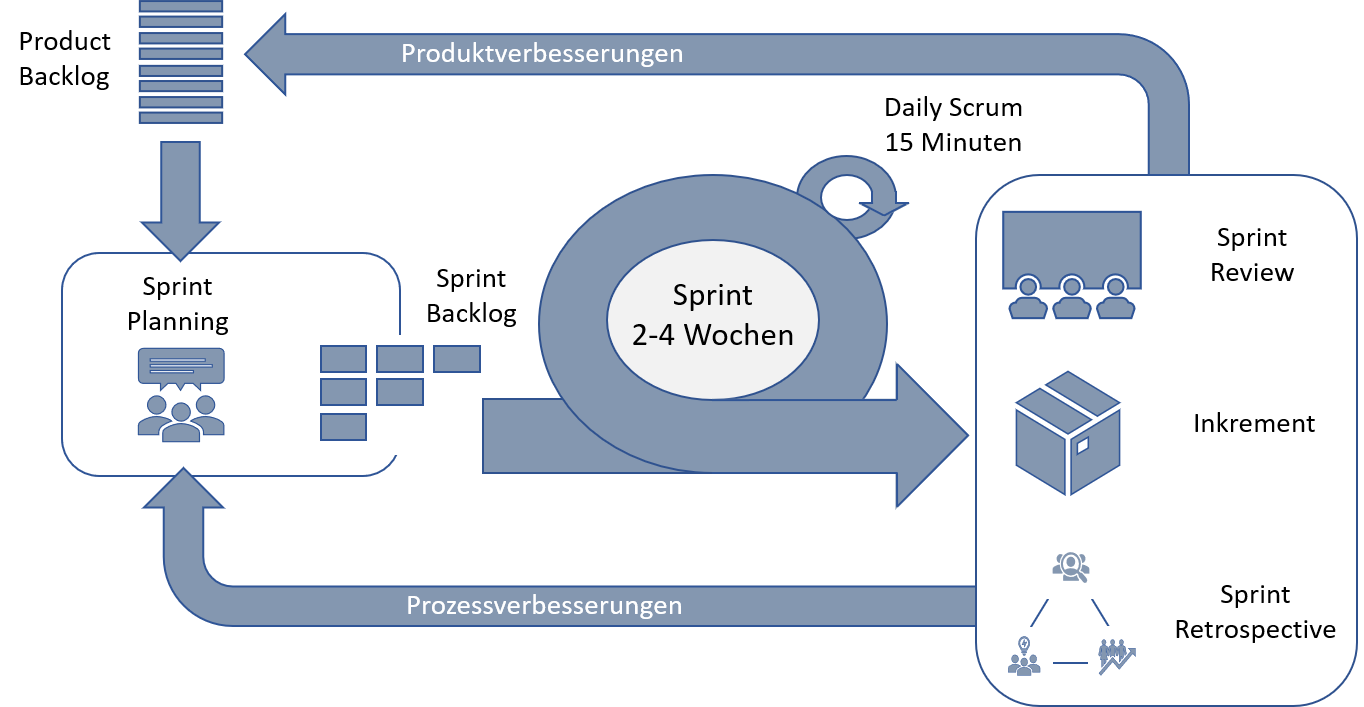
\includegraphics[width=1.0\textwidth]{06_Bilder/Scrum_prozess.png}
	\setlength{\abovecaptionskip}{1em}
	\caption{Scrum-�berblick in Anlehnung an \autocite[][S.38 Abb.3.6]{agiles_pm_berufsalltag}}
	\label{img:scrum_prozess}
\end{figure}

Mithilfe der Rollen, Artefakte und Events l�sst sich schon ein grobes Bild des Scrum Prozesses erstellen. In Abbildung \ref{img:scrum_prozess} ist der gesamte Scrum Prozess abgebildet. Dieser startet beim Sprint Planning. Dort bespricht das Team wie viele und welche To-dos aus dem Product Backlog im n�chsten Sprint abzuarbeiten sind. Am Ende des Meetings werden alle vereinbarten To-dos vom Development Team in Tasks heruntergebrochen, an ein Board gehangen und somit das Sprint Backlog erstellt \autocite[vgl.][S.34-42]{agiles_pm_berufsalltag}. 
\\\\
W�hrend des sprints, wird am erfolgreichen Abschluss der Tasks gearbeitet. Durch das t�gliche  Daily Scrum Meeting werden Probleme erfasst, die das Development Team daran hindern, Tasks erfolgreich abzuschlie�en. Zus�tzlich gewinnen alle Teammitglieder einen �berblick �ber den momentanen Stand der Arbeit \autocite[vgl.][S.34-42]{agiles_pm_berufsalltag}. 
\\\\
Nach Abschluss des sprints, wird das Ergebnis (Inkrement) w�hrend des Sprint Review Meetings vorgestellt. Hier werden Verbesserungsvorschl�ge und Feedback gesammelt, die wiederum in das Product Backlog mit aufgenommen werden. Zus�tzlich wird das Sprint Retrospective Meeting abgehalten, dass das Ziel hat, den letzten Sprint zu reflektieren, um die Zusammenarbeit zu optimieren und den Prozess zu verbessern. Anschlie�end startet der Prozess wieder beim Sprint Planning \autocite[vgl.][S.34-42]{agiles_pm_berufsalltag}.

  
\newpage
\subsection{Kanban} \label{Kap:Kanban}
Urspr�nglich wurde Kanban zur Steuerung des Materialflusses innerhalb der Produktion entwickelt. Der Begriff Kanban hat in der englischen Literatur zwei unterschiedliche Bedeutungen, je nachdem ob dieser gro�- oder kleingeschrieben ist. Die Methode wird gro�geschrieben, hingegen als Signalkarte, System und Board klein. Im deutschen Sprachgebrauch wird vereinfacht nur von \enquote{Kanban} gesprochen \autocite[vgl.][S.42]{agiles_pm_berufsalltag}.
\\\\
In dieser Arbeit wird Kanban nicht zur Steuerung des Materialflusses genauer erl�utert, sondern die abgewandelte Version zur Softwareentwicklung. Diese wurde im Jahre 2007 von David J. Anderson entwickelt \autocite[vgl.][S.1]{kanban}. 




\section{Agilit\"at in gro�en Unternehmen} \label{Kap:AgilitaetGrosseUnternehmen}
Was f�r Formen werden in gro�en Teams verwendet? SCRUM in SCRUM? usw.. Recherche!

\section{Klassische Projektmanagementmethoden} \label{Kap:KlassischeProjektmanagementmethoden}
Klassische Projektmanagementmethoden
V Modell?
Wasserfall?
G�ngigste Methoden herausfinden und definieren. (Evtl. darauf achten welche Methoden die Unternehmen sp�ter in den Berichten und Interviews verwenden und diese hier erl�utern)

\section{Agile Transformation} \label{Kap:AgileTransformation}
Was ist die Agile Transformation? Bitte IT Kontext beibehalten!




% !TEX root = UnternehmensEinteilung.tex

\chapter{Einteilung der Unternehmen}
Um im sp�teren Verlauf die Herausforderungen f�r bestimmte Unternehmensarten abgrenzen zu k�nnen, m�ssen diese erst definiert werden. Jede Art eines Unternehmens besitzt pr�gnante Merkmale, die die Zugeh�rigkeit zu einer bestimmten Art bestimmen. Einigen Lesern werden die Begriffe Startup, Mittelstand und Konzern vertraut sein. Welche pr�gnanten Merkmale diese Arten genau definieren, d�rfte allerdings den wenigsten Menschen gel�ufig sein. In diesem Kapitel werden die verschiedenen Arten von Startup �ber den Mittelstand bis hin zum Konzern definiert und die daraus resultierenden pr�gnanten Merkmale festgelegt. 

\section{Startup} \label{Kap:Startup}
\begin{definition}{Definition Startup (Quelle: \autocite{definition_startup})}{def:startup}
	\\ 
	Junge, noch nicht etablierte Unternehmen, die zur Verwirklichung einer innovativen Gesch�ftsidee (h�ufig in den Bereichen Electronic Business,	Kommunikationstechnologie oder Life Sciences) mit geringem Startkapital gegr�ndet werden und i.d.R. sehr fr�h zur Ausweitung ihrer Gesch�fte und	St�rkung ihrer Kapitalbasis entweder auf den Erhalt von \gls{venturecapital} bzw. Seed Capital (evtl. auch durch Business Angels) angewiesen sind.
	Aufgrund der Aufnahme externer Gelder wie Venture-Capital ist das Unternehmen auf einen Exit angewiesen, im Zuge dessen die Kapitalgeber ihre Investments realisieren.
	\\
\end{definition}

Auf Basis der Definition lassen sich folgende pr�gnante Merkmale herauskristallisieren:

\begin{itemize}
	\item Das Unternehmen wurde erst vor wenigen Monaten oder Jahren gegr�ndet
	
	\item Der Fokus liegt auf der Verwirklichung einer innovativen Gesch�ftsidee
	
	\item Geringes Startkapital bei der Gr�ndung
	
	\item Aufgrund der Aufnahme externer Gelder, entsteht eine Erwartungshaltung gegen�ber den Investoren
\end{itemize}

Die Definition und die daraus resultierenden pr�gnanten Merkmale zeigen, das der allgemeing�ltige Gedanke, Startups sind kleine Unternehmen, die erst vor kurzer Zeit gegr�ndet wurden, teilweise stimmig ist. Zus�tzlich geht hervor das Startups sehr stark auf die Aufnahme externer Gelder angewiesen sind. Aus diesen Gr�nden l�sst sich ableiten, dass der Druck eine Innovation zu realisieren hoch ist, da die Kapitalgeber in diese investieren. Zus�tzlich liegt der Fokus auf der Verwirklichung einer innovativen Gesch�ftsidee, was h�ufig eine Kultur des engen Zusammenhalts und einer gemeinschaftlichen Arbeitsweise herbeif�hrt. 
\\\\
Des Weiteren ist anzumerken, dass Startups die besten Voraussetzungen f�r ein gut funktionierendes Projektmanagement besitzen, da die Unternehmensgr��e noch relativ �berschaubar ist. Dadurch k�nnen diese flexibel auf neue Situationen reagieren \autocite[vgl.][]{pragmatisches_pm_f_startups}.

\section{Mittelstand} \label{Kap:Mittelstand}
Laut \autocite{definition_mittelstand} gibt es keine allgemeing�ltige Definition f�r den Begriff Mittelstand. Der Begriff kann jedoch anhand g�ngiger Definitionen abgegrenzt werden, um quantitative und qualitative Merkmale zu erhalten. H�ufig wird der Begriff \acs{KMU} (kleine und mittlere Unternehmen) verwendet, der der englischen Abk�rzung \acs{SME} (small and medium sized enterprise) nachempfunden ist. Eine der g�ngigsten Abgrenzungen f�r den Begriff des deutschen Mittelstands ist die des \enquote{Instituts f�r Mittelstandsforschung Bonn} (folgend \acs{IFM} Bonn genannt). Da das \acs{IFM} Bonn Unternehmen anhand von quantitativen Kriterien wie Jahresumsatz und Besch�ftigtenzahl definiert, wird diese Abgrenzung als quantitativer Teil zur Definition des Mittelstands verwendet \autocite[vgl.][]{definition_mittelstand}.
% Tabelle
\begin{table}[H]
	\centering
	\begin{tabular}{|l|c|c|}
		\hline
		\textbf{Unternehmensgr��e}	& \textbf{Zahl der Besch�ftigten}	& \textbf{Umsatz \euro/Jahr} \\ \hline
		kleinst	& bis 9		& bis 2 Millionen		\\
		klein	& bis 49    & bis 10 Millionen	 	\\
		mittel 	& bis 499 	& bis 50 Millionen		\\ \hline
		\textbf{KMU zusammen}	& \textbf{unter 500}	& \textbf{bis 50 Millionen} \\
		\hline
	\end{tabular}
	
	\caption{KMU-Definition in Anlehung an \autocite{definition_mittelstand} und \autocite{definition_mittelstand2}}
	\label{tbl:IFM_KMU_definition}
	
\end{table}

Quantitativ kann auf Basis der Tabelle \ref{tbl:IFM_KMU_definition} ein mittelst�ndisches Unternehmen bis zu 500 Mitarbeiter besch�ftigen und 50 Millionen Euro Umsatz im Jahr generieren. Qualitativ weisen mittelst�ndische Unternehmen die folgenden Merkmale auf (qualitative Ziele nach \autocite{definition_mittelstand2}):

\begin{itemize}
	\item Einheit von Eigentum, Haftung und F�hrung
	
	\item Bis zu zwei nat�rliche Personen oder ihre Familienangeh�rigen (direkt oder indirekt) halten mindestens 50 \% der Anteile eines Unternehmens
	
	\item diese nat�rlichen Personen (Anteilshaber) geh�ren der Gesch�ftsf�hrung an
\end{itemize}

Auf Basis der quantitativen und qualitativen Kriterien k�nnen die folgenden pr�gnanten Merkmale, die ein mittelst�ndisches Unternehmen definieren, abgeleitet werden:

\begin{itemize}
	\item Bis zu 500 Mitarbeiter sind im Unternehmen besch�ftigt
	
	\item Bis zu 50 Millionen Euro Umsatz pro Jahr
	
	\item Bis zu zwei nat�rliche Personen oder ihre Familienangeh�rigen (direkt oder indirekt) halten mindestens 50 \% der Anteile eines Unternehmens
	
	\item Anteilshaber geh�ren der Gesch�ftsf�hrung an
\end{itemize}

Aus den pr�gnanten Merkmalen geht hervor, dass mittelst�ndische Unternehmen oft famili�re Strukturen aufweisen. Aus diesem Grund sind h�ufig flache Hierarchien aufzufinden. Das f�rdert ein flexibles Vorgehen und eine schnelle Entscheidungsfindung \autocite[vgl.][]{projektmanagement_mittelstand}.

\section{Konzern} \label{Kap:Konzern}

\begin{definition}{Definition Begriff Konzern (Quelle: \autocite{definition_konzern})}{def:Konzern}
	\\ 
	Sind ein herrschendes und ein oder mehrere abh�ngige Unternehmen unter der einheitlichen Leitung des herrschenden Unternehmens zusammengefasst, so bilden sie einen Konzern. Die einzelnen Unternehmen sind Konzernunternehmen. Liegt ein Beherrschungsvertrag oder eine Eingliederung vor, sind die Unternehmen als unter einheitlicher Leistung zusammengefasst anzusehen. Sind rechtlich selbstst�ndige Unternehmen, ohne dass das eine Unternehmen von dem anderen abh�ngig ist, unter einheitlicher Leitung zusammengefasst, bilden auch sie einen Konzern.
	\\
\end{definition}

Aus der Definition (siehe Definition Begriff Konzern) geht hervor, dass ein Konzern ein Gebilde aus mehreren Unternehmen ist. Dabei agiert ein Unternehmen als \enquote{Herrschendes} und ein oder mehrere Unternehmen ordnen sich unter. Zusammen bilden sie einen Konzern. So lassen sich die folgenden pr�gnanten Merkmale f�r einen Konzern wie folgt schildern:

\begin{itemize}
	\item Ein Unternehmen agiert als \enquote{herrschendes} Unternehmen
	
	\item Mehrere Unternehmen ordnen sich unter
	
	\item Untergeordnete Unternehmen k�nnen auch rechtlich selbstst�ndige Unternehmen sein
\end{itemize}

Da ein Konzern mehrere Unternehmen vereint, sind die Hierarchien entsprechend hoch. Dieser Umstand macht es schwierig eine Kultur des engen Zusammenhalts und einer gemeinschaftlichen Arbeitsweise, wie es etwa bei Startups h�ufig der Fall ist (siehe Kapitel \ref{Kap:Startup} Startup), beizubehalten. Zus�tzlich erschwert es ein flexibles Vorgehen und eine schnelle Entscheidungsfindung im Vergleich mit mittelst�ndischen Unternehmen.
\\\\
Zusammengefasst besitzt jede Unternehmensart pr�gnante Merkmale, die das jeweilige Unternehmen definieren. Startups sind h�ufig sehr junge Unternehmen mit einer innovativen Gesch�ftsidee. Der Mittelstand auf qualitativer Ebene eher traditionell und famili�r gepr�gt und auf quantitativer Ebene mitarbeiter- und umsatzbezogen. Konzerne hingegen sind gro�e Unternehmenskomplexe, in denen sich viele Unternehmen einer Hierarchie unterordnen. Im n�chsten Kapitel werden Berichte und Interviews �ber die agile Transformation verschiedener Unternehmen analysiert. Da nun pr�gnante Merkmale zur Identifikation der verschiedenen Unternehmensarten geschaffen wurden, k�nnen im n�chsten Kapitel die Berichte und Interviews den verschiedenen Unternehmensarten zugeordnet werden. Dies ist wichtig im weiteren Verlauf um eventuelle Zusammenh�nge hinsichtlich der Herausforderung der agilen Transformation herauszufinden.  

% !TEX root = Erfahrungen.tex

\chapter{Erfahrungen der Agilen Transformation}

In den vorherigen Kapiteln wurde erl�utert, was der Begriff der agilen Transformation f�r Unternehmen bedeutet und welche verschiedenen Unternehmensarten es gibt. Dieses Kapitel soll Erfahrungen bereits durchgef�hrter Transformationen in Form von Berichten zusammentragen. Zus�tzlich werden verschiedene Mitarbeiter, verschiedener Unternehmen zu dem Thema befragt. Das Ziel dieses Kapitels ist die Ermittlung verschiedenster Herausforderungen durch eine Analyse der Berichte und Interviews. 

\section{Berichte} \label{Kap:Berichte}
Es gibt einige Unternehmen und Berater, die sich mit dem Thema der agilen Transformation bereits auseinandergesetzt haben. Jeder hat dabei seine eigenen Erfahrungen gemacht. Diese werden im Folgenden dargelegt.

\subsubsection{Erfahrungsbericht eines agilen Beraters \autocite[vgl.][]{erfahrungsbericht1}}

Desto gr��er eine Organisation ist, desto tr�ger ist diese. Ein einziges Problem wird h�ufig mit vielen verschiedenen \glspl{workaround} und individuellen L�sungen behoben. Zus�tzlich gibt es wenig Kooperation zwischen den verschiedenen Bereichen, was zu verlorenen Wissen f�hrt. Das hat zur Folge das Priorit�ten falsch gesetzt und Projekte verz�gert werden. Dieses Problem wird zus�tzlich durch anspruchsvollere Kunden und Mitarbeiter, komplexere Projekte und die Digitalisierung verst�rkt. Um diese Herausforderungen zu bew�ltigen, m�chten viele Unternehmen agil werden.
\\\\
Als Unternehmen zu erkennen, was �berhaupt mit der \enquote{Agilit�t} erreicht werden will, ist eine der Herausforderungen der Transformation. Ist es mehr Transparenz in Projekten oder eher Geschwindigkeit und Effizienz, die angestrebt werden. Wie auch immer die Ziele der Transformation aussehen, es muss immer im Vorhinein der Aufwand dem Gegenwert gegen�bergestellt werden.  
\\\\
Konzerne besitzen eine v�llig andere Gr��enordnung im Vergleich zu Startups. Konzernabteilungen agieren weitestgehend unabh�ngig voneinander und besitzen eigene Budgets. Zus�tzlich sind diese r�umlich voneinander getrennt und Besitzen klare hierarchische Strukturen. Dabei spielt es eine gro�e Rolle Wertsch�pfung eindeutig zuzuordnen. Viele Unternehmen haben w�hrend der agilen Transformation Probleme, �berhaupt einzusch�tzen, ob die agilen Ziele Vorrang vor den klassischen haben. 
\\\\
Besonders bei der Umsetzung der agilen Methoden und der Transformation ist die \acs{IT} gefragt. Diese ertrinkt jedoch h�ufig zus�tzlich im Tagesgesch�ft. Damit die Transformation nicht endlos wird, werden einige Grundvoraussetzungen ben�tigt. Die Umwandlung der Organisation ist hier zus�tzlich eine Belastung, da das Gesch�ft weiter gehen muss, w�hrend es transformiert wird. Zus�tzlich ergibt es keinen Sinn, gleich alle Bereiche umzuwandeln.  
\\\\
Es wird ein gro�es Konzept ben�tigt, innerhalb dem kleine agile Teams arbeiten k�nnen, allerdings trotzdem Anforderungen des Business erf�llt werden k�nnen. In manchen F�llen wird hierf�r die gesamte Arbeitskultur aufgebrochen, h�ufig gen�gt es, bei einzelnen Bereichen anzufangen. Die gesamte Arbeitsweise muss ge�ndert werden um die Bereitschaft zur Agilit�t hinzuschaffen. Um diese Bereitschaft zu schaffen, muss bei der Ver�nderung des Verg�tungs- und Aufstiegsmodells angefangen werden, bis hin zur Aufstellung der Teams. Das Klima innerhalb der Organisation muss Offenheit und die Bereitschaft sich, ohne Grenzen auszutauschen, f�rdern. F�r gro�e Organisationen ist das h�ufig nicht in einem Schritt zu schaffen.
\\\\
Konzernprojekte werden h�ufig unternehmensweit geplant. Die Teams arbeiten agil an kleinen Aufgaben mit klar definierten Ergebnissen. Zus�tzlich sind sie immer �ber das gr��ere Ziel und den Status der anderen Teams gut informiert. Werden Abteilungen im Zuge der Transformation zu \gls{coredeliverable} Areas, so m�ssen diese pl�tzlich Produkte und Services in planbare Einheiten herunterbrechen. Alle Teams und �bergreifenden Gruppen m�ssen jetzt Abh�ngigkeiten und Risiken jedes Zeitpunkts im Lebenszyklus im Blick behalten. In der Praxis allerdings ist es nicht so einfach, an diesen Punkt zu kommen. Die Gewohnheit der Teams lag darin, in abgeschlossenen Einheiten zu arbeiten und ihre kleineren eigenen Ziele im Auge zu behalten. Des Weiteren m�ssen diese sich erst an die Aufwandsmessung in Story Points statt Mann-Tagen gew�hnen. H�ufig f�hrt diese Umstrukturierung zu langen Diskussionen. Eine sinnvolle Interaktion zwischen den Teams und eine weitergehende Transparenz muss erst ge�bt werden.
\\\\  
Ein weiterer Aspekt ist die technologische Ebene. Problematisch wird ein einheitliches Projektmanagement wenn die Teams keine einheitliche Technologie zur Schaffung von Transparenz und zur Arbeitsplanung verwenden. Die Einf�hrung solcher Teams muss durch Trainings w�hrend der Einf�hrung unterst�tzt werden. Der Prozess ist iterativ mit Einfluss des gesamten Feedbacks. Um eine einzige Wahrheit als Basis f�r die Planung, Umsetzung, Testing, Release Management und das Reporting zu schaffen, m�ssen alle Tools auf den gleichen Datenpool zugreifen. 
\\\\
Ein gro�er Kunde von uns nutzt CA Agile Central. Das Planungstool wurde extra f�r die Anforderungen des Konzerns entworfen und hilft dem Kunden bei \gls{cicd} and Delivery oder \gls{devops}. Als erstes Pilotprojekt beschr�nkte sich das Tool zun�chst auf eine Niederlassung. Eines der Probleme waren die niederlassungs�bergreifenden Strukturen in ein agiles Projekt miteinzubeziehen und diese umzuwandeln. Einer der entscheidenden Faktoren war, dass seit Beginn auf Konzernleitungsebene eine gro�e Aufmerksamkeit bestand und aktiv seitens Niederlassungsleitung unterst�tzt wurde. Besonders geholfen hat es, einzelne als Botschafter f�r den agilen Ansatz zu machen. Diese Botschafter sollten sicherstellen, dass Botschaften konsistent bleiben und Regeln eingehalten werden.

\section{Interviews} \label{Kap:Interviews}
Unternehmen, Menschen oder Internet evtl. auch B�cher

\section{Analyse} \label{Kap:Analyse}
Welche Merkmale und Schwierigkeiten haben sich w�hrend der Berichte und Interviews herauskristallisiert?



% !TEX root = Herausforderungen.tex

\chapter{Herausforderungen}

In Kapitel \ref{Kap:Analyse} wurden Herausforderungen und Metainformationen der jeweiligen Unternehmenstypen ermittelt. In diesem Kapitel werden alle ermittelten Herausforderungen hinsichtlich der Unternehmenstypen Startup, Mittelstand und Konzern betrachtet. Die Herausforderungen werden jeweils bewertet, wie Schwerwiegend diese f�r die agile Transformation des jeweiligen Unternehmenstyps sind. Nachdem ermittelt wurde, was die schwerwiegendsten Herausforderungen sind, werden Ratschl�ge zur Beseitigung dieser aufgef�hrt. Ziel dieses Kapitels ist es, dem Leser zu vermitteln, was genau Unternehmen davon abh�lt, eine agile Transformation durchzuf�hren. Im folgenden werden die Herausforderungen und Metainformationen nicht mehr aufgef�hrt und nur noch anhand ihrer Nummer aufgef�hrt. Diese k�nnen dem Kapitel \ref{Kap:Ergebnisse} Ergebnisse vollst�ndig entnommen werden.

\section{Zuordnung nach Unternehmenstyp} \label{Kap:ZuordnungSchwierigkeiten}
Im ersten Schritt werden alle ermittelten Herausforderungen (siehe Kapitel \ref{Kap:Ergebnisse}) aus der Sicht des jeweiligen Unternehmenstyps betrachtet. Dabei wird entschieden, ob die Herausforderung �berhaupt auf den Unternehmenstyp zutrifft und wie Schwerwiegend die Auswirkungen auf die agile Transformation sind. Die ebenfalls in Kapitel \ref{Kap:Ergebnisse} ermittelten Metainformationen werden zus�tzlich zur Betrachtung verwendet.
\\\\
Um eine bessere �bersicht zu vermitteln, wie schwerwiegend eine Herausforderung f�r den jeweiligen Unternehmenstyp hinsichtlich der agilen Transformation ist, wird ein Ampelsystem verwendet. Dieses sieht wie folgt aus:

\begin{itemize}
	\item [\textcolor{red}{\Huge\textbullet}] \textbf{- Rot, Schwerwiegend}\\Gef�hrdet die agile Transformation und ist schwierig zu l�sen
	\item [\textcolor{orange}{\Huge\textbullet}] \textbf{- Orange, Normal}\\Gef�hrdet die agile Transformation und l�sst sich einfach l�sen
	\item [\textcolor{green}{\Huge\textbullet}] \textbf{- Gr�n, Leicht}\\Gef�hrdet kaum die agile Transformation und l�sst sich einfach l�sen
\end{itemize}

\newpage
\subsection{Startup}

Zur Zuordnung und Bewertung, werden die Metainformationen der Tabelle \ref{tbl:ergebnisse_startups} verwendet. Zus�tzlich k�nnen Begr�ndungen auch auf Basis der ermittelten Daten aus aus Kapitel \ref{Kap:Erfahrungen} oder anhand von Logik gebildet werden.

\setlength\LTleft{-1in}
\setlength\LTright{-1in}
\begin{longtable}{|p{1,1cm}|p{1,5cm}|p{15,9cm}|}
	\caption{Startup - Bewertung der Herausforderungen} \label{tbl:bewertung_startup} \\
	
	\hline \multicolumn{1}{|c|}{\textbf{Hf.}} 
	& \multicolumn{1}{c|}{\textbf{Bew.}}
	& \multicolumn{1}{c|}{\textbf{Begr�ndung}} \\ \hline 
	\endfirsthead
	
	\multicolumn{3}{c}%
	{{\bfseries \tablename\ \thetable{} -- weiterf�hrend von letzter Seite}} \\
	\hline \multicolumn{1}{|c|}{\textbf{Hf.}} 
	& \multicolumn{1}{c|}{\textbf{Bew.}}
	& \multicolumn{1}{c|}{\textbf{Begr�ndung}} \\ \hline 
	\endhead
	
	\hline \multicolumn{3}{|r|}{{Wird auf der n�chsten Seite weitergef�hrt}} \\ \hline
	\endfoot
	
	\hline \hline
	\endlastfoot
	
	\hyperlink{k11}{K1.1} & \cellcolor{orange}
	& Aufgrund der noch �berschaubaren Unternehmensgr��e, l�sst sich noch gut reflektieren, was mit einer agilen Transformation erreicht werden m�chte.
	\\ \hline
	\hyperlink{k12}{K1.2} & \cellcolor{orange}
	& Startups sind h�ufig relativ junge Unternehmen. Aus diesem Grund lassen sich Ziele noch einfacher anpassen als beispielsweise bei �lteren Unternehmen mit bereits ausgepr�gteren Zielen.
	\\ \hline
	\hyperlink{k13}{K1.3} & \cellcolor{orange}
	& Wenn das Tagesgesch�ft nicht mehr weitergef�hrt werden kann, ist das Schwerwiegend f�r das Unternehmen. Da Startups h�ufig keine festen Teamgrenzen besitzen (siehe \hyperlink{k23}{K2.3}), entsteht h�ufig eine \enquote{Jeder macht und kann alles Mentalit�t}. Aus diesem Grund f�llt es den Mitarbeiter leichter, Priorit�ten hinsichtlich des Tagesgesch�fts einzusch�tzen.
	\\ \hline
	\hyperlink{k14}{K1.4} & \cellcolor{green}
	& Da Startups h�ufig neue und innovative Wege mit jedem Projekt gehen (siehe \hyperlink{k21}{K2.1}), ist die Anpassungsf�higkeit der Mitarbeiter ausgepr�gter.
	\\ \hline
	\hyperlink{k15}{K1.5} & \cellcolor{green}
	& Startups die nicht abh�ngig von einem Mutterkonzern sind, haben h�ufig wenig Schnittpunkte. Aus diesem Grund sind oft nicht so viele Abh�ngigkeiten vorhanden an die sich die Teams gew�hnen m�ssen. Auch hier d�rfte zus�tzlich der Faktor, dass die Mitarbeiter daran gew�hnt sind neue und innovative Wege mit jedem Projekt zu gehen eine Rolle spielen (siehe \hyperlink{k21}{K2.1}).
	\\ \hline
	\hyperlink{k16}{K1.6} & \cellcolor{green}
	& Da es in Startups h�ufig keine festen Teamgrenzen gibt (siehe \hyperlink{k23}{K2.3}), �bernehmen Teams schon fr�h Verantwortung. Im Zuge der Transformation d�rfte somit diese Herausforderung kaum eine Rolle spielen.
	\\ \hline
	\hypertarget{B17}{\hyperlink{k17}{K1.7}} & \cellcolor{green}
	& Der Aspekt, dass Mitarbeiter aufgrund der geringeren Mitarbeiteranzahl fr�h Verantwortung �bernehmen m�ssen, spielt hierbei eine gro�e Rolle. Mitarbeiter m�ssen schon vor der Transformation lernen sich selbst zu organisieren und die Toleranz gegen�ber dem Management einfordern.
	\\ \hline
	\hyperlink{k18}{K1.8} & \cellcolor{orange}
	& Wenn die Mitarbeiter nicht gen�gend geschult werden, gef�hrdet das die Transformation, da die Werte, Prinzipien und Methoden falsch verstanden werden. Die �berschaubare Unternehmensgr��e eines Startups, l�sst es zu, dass Mitarbeiter sich schnell austauschen und fr�h, Mitarbeiter gut geschult werden k�nnen.
	\\ \hline
	\hyperlink{k19}{K1.9} & \cellcolor{green}
	& Da Startups noch relativ junge Unternehmen sind, m�ssen h�ufig erst Strukturen gebildet werden.
	\\ \hline
	\hyperlink{k110}{K1.10} & \cellcolor{green}
	& Es ist davon auszugehen, dass eine gute Feedbackkultur einfach in Startups einzuf�hren ist, da diese Unternehmen sich permanent anpassen und ver�ndern (siehe \hyperlink{k25}{K2.5}).
	\\ \hline
	\hyperlink{k111}{K1.11} & \cellcolor{orange}
	& Diese Herausforderung kann schwerwiegend f�r die agile Transformation sein. Startups wandeln sich permanent und k�nnen h�ufig agile Projekte besser integrieren (siehe \hyperlink{k25}{K2.5}).
	\\ \hline
	\hyperlink{k112}{K1.12} & \cellcolor{orange}
	& Jedes Unternehmen muss selber absch�tzen ob klassisch oder agil der bessere Weg f�r das Unternehmen ist.
	\\ \hline
	\hyperlink{k113}{K1.13} & \cellcolor{orange}
	& Wenn Mitarbeiter ein falsches Verst�ndnis von Agilit�t besitzen, kann das schwerwiegend f�r die agile Transformation sein. In Startups l�sst sich dieser Umstand durch gute Schulungen und eine entsprechende Unternehmenskultur verbessern.
	\\ \hline
	\hyperlink{k114}{K1.14} & \cellcolor{orange}
	& Teams in Startups haben durch die geringe Unternehmensgr��e (flache Hierarchien) schon vor der Transformation eine hohe Verantwortung.
	\\ \hline
	\hyperlink{k115}{K1.15} & \cellcolor{green}
	& Startups m�ssen sich permanent anpassen und ver�ndern. Zus�tzlich l�sst sich relativ einfach, aufgrund der noch geringen Mitarbeiteranzahl die Kultur anpassen.
	\\ \hline
	\hyperlink{k116}{K1.16} & \cellcolor{green}
	& Startups m�ssen sich permanent anpassen und wandeln (siehe ). Dieser Umstand macht es Mitarbeitern leichter, sich an neue Prozesse zu gew�hnen (siehe \hyperlink{k25}{K2.5}).
	\\ \hline
	\hyperlink{k117}{K1.17} & \cellcolor{green}
	& Aufgrund der geringen Mitarbeiteranzahl, m�ssen Mitarbeiter schon fr�h lernen sich selbst zu organisieren. 
	\\ \hline
	\hyperlink{k118}{K1.18} & \cellcolor{green} 
	& Startups f�llt es leichter die interne Organisation zu fixieren, bei stetig wechselnder Projektteams, da diese sich permanent anpassen und ver�ndern und oft neue Technologien und Methoden annehmen (siehe \hyperlink{k25}{K2.5} \& \hyperlink{k24}{K2.4}).
	\\ \hline
	\hyperlink{k119}{K1.19} & \cellcolor{orange}
	& Startups m�ssen sich permanent anpassen und ver�ndern (siehe \hyperlink{k25}{K2.5}).
	\\ \hline
	\hyperlink{k120}{K1.20} & \cellcolor{red}
	& Da Startups sich permanent anpassen und ver�ndern, nehmen diese auch h�ufig neue Technologien und Methoden an (siehe \hyperlink{k25}{K2.5} \& \hyperlink{k24}{K2.4}). Wenn nicht darauf geachtet wird, nur sinnvolle technische Neuerungen zu implementieren, kann dies die Transformation aufgrund von unn�tigen Investitionen und Mitarbeiterdemotivation gef�hrden. 
	\\ \hline
	\hyperlink{k121}{K1.21} & \cellcolor{red}
	& Da Startups sich permanent anpassen und ver�ndern (siehe \hyperlink{k25}{K2.5}), besteht hier eine erh�hte Gefahr den Fokus auf das wesentliche zu verlieren.
	\\ \hline
	\hyperlink{k122}{K1.22} & \cellcolor{orange}
	& Trends zu beobachten ist einer der essenziellen Erfolgsfaktoren eines Startups. 
	\\ \hline
	\hyperlink{k123}{K1.23} & \cellcolor{red}
	& Startups die in Konzerne eingebettet sind, haben viele Schnittpunkte zu ihrem Mutterkonzern. Dies kann die agile Transformation erheblich beeintr�chtigen, wenn diese unterschiedliche Strukturen und Kulturen besitzen.
	\\ \hline
	\hyperlink{k124}{K1.24} & \cellcolor{green}
	& Startups besitzen meist eine flache Hierarchie. 
	\\ \hline
	\hyperlink{k125}{K1.25} & \cellcolor{green}
	& Aufgrund der kaum vorhandenen Teamgrenzen (siehe \hyperlink{k23}{K2.3}), ist ein hoher Austausch von Informationen unter den Mitarbeitern vorhanden. Dies hat den Vorteil das Werte gut vermittelt werden k�nnen.
	\\ \hline
	\hyperlink{k126}{K1.26} & \cellcolor{red}
	& Startups sind auf ihr Kapital angewiesen, da diese im Wachstum sind. Wenn das Kapital knapp wird, besteht die Gefahr, dass die agile Transformation nicht weitergef�hrt wird.
	\\ \hline
	\hyperlink{k127}{K1.27} & \cellcolor{green}
	& Aufgrund der flachen Hierarchien lassen sich externe Mitarbeiter sehr gut eingliedern.
	\\ \hline
	\hyperlink{k128}{K1.28} & \cellcolor{red}
	& Aufgrund der starken Abh�ngigkeit zu den Kapitalgebern (siehe Kapitel \ref{Kap:Startup}), kann es passieren, dass Gegner die agile Transformation gef�hrden.
	\\ \hline
	\hyperlink{k129}{K1.29} & \cellcolor{green}
	& Mitarbeiter besitzen aufgrund der geringen Mitarbeiteranzahl schon vor der agilen Transformation viel Verantwortung.
	\\ \hline
	\hyperlink{k130}{K1.30} & \cellcolor{green}
	& Da Startups junge Unternehmen sind (siehe Kapitel \ref{Kap:Startup}), lassen sich einfacher Vorzeigeprojekte durchf�hren.
	\\ \hline
	\hyperlink{k131}{K1.31} & \cellcolor{orange}
	& Da Startups junge Unternehmen sind (siehe Kapitel \ref{Kap:Startup}), lassen sich Prozesse noch einfacher definieren und anpassen. 
	\\ \hline
	\hyperlink{k132}{K1.32} & \cellcolor{orange}
	& Bereits bestehende langfristige klassische Projekte d�rften kaum in Startups vorhanden sein, da diese meist relativ jung sind.
	\\ \hline
	\hyperlink{k133}{K1.33} & \cellcolor{green}
	& Da Startups sich permanent anpassen und ver�ndern m�ssen (siehe \hyperlink{k25}{K2.5}), f�llt es den Mitarbeitern leichter, ihr Mindset zu ver�ndern.
	\\ \hline
	\hyperlink{k134}{K1.34} & \cellcolor{green} 
	& Diese Herausforderung motiviert Mitarbeiter in Startups, da den Geldgebern fr�h vorzeigbare Ergebnisse geliefert werden.
	\\ \hline
	\hyperlink{k135}{K1.35} & \cellcolor{green}
	& Durch die flache Hierarchie und den hohen Informationsaustausch sind die Vorteile einer guten Fehlerkultur fr�h zu erkennen.
	\\ \hline
	\hyperlink{k136}{K1.36} & \cellcolor{green}
	& Es bestehen oft keine festen Teamgrenzen, was den Austausch von Informationen erleichtert. 
	\\ \hline
	\hyperlink{k137}{K1.37} & Keine Bewertung m�glich
	& Startups sind keine traditionellen Unternehmen, da diese sehr jung sind (siehe Kapitel \ref{Kap:Startup})
	\\ \hline
	\hyperlink{k138}{K1.38} & \cellcolor{green}
	& Durch die flachen Hierarchien, ist es einfacher, Mitarbeitern die Angst vor Fehlern zu nehmen. 
	\\ \hline
	\hyperlink{k139}{K1.39} & Keine Bewertung m�glich
	& Startups haben kaum Erfahrungswerte, da diese sehr jung sind (siehe Kapitel \ref{Kap:Startup})
	\\ \hline
	\hyperlink{k140}{K1.40} & \cellcolor{orange}
	& Da Startups stark auf ihre Kapitalgeber angewiesen sind, m�ssen h�ufig fr�h vorzeigbare Ergebnisse geliefert werden. Je nach Kapitalgeber, kann es sein das durch diesen Umstand, Startups gezwungen werden, Deadlines zu definieren.
	\\ \hline
	\hyperlink{k141}{K1.41} & \cellcolor{orange}
	& Startups sind sehr junge Unternehmen. Aus diesem Grund fehlt h�ufig der Vergleich komplett. Das kann Auswirkungen auf die agile Transformation haben, da somit eine Argumentationsgrundlage fehlt.
	\\ \hline
	\hyperlink{k142}{K1.42} & \cellcolor{red}
	& Subjektive Meinungen k�nnen h�chstens mithilfe von Argumentationsgrundlagen ge�ndert werden. Diese sind bei einem jungen Unternehmen ohne Erfahrungswerte h�ufig nicht vorhanden.
	\\ \hline
	\hyperlink{k143}{K1.43} & \cellcolor{green}
	& Da Startups junge Unternehmen sind, ist die Kultur und der Umgang miteinander im stetigen wandel.
	\\ \hline
	\hyperlink{k144}{K1.44} & \cellcolor{orange}
	& Startups m�ssen sich permanent anpassen und ver�ndern. Solange das Unternehmen noch jung ist, lassen sich Prozesse einfacher anpassen.
	\\ \hline
	\hyperlink{k145}{K1.45} & \cellcolor{orange}
	& Wenn Mitarbeiter nicht die Vorteile der Agilit�t erkennen, ist es schwer diese anzunehmen und umzusetzen. Dieser Umstand l�sst sich nur durch gute Schulungen und vorhergegangene Projekte beheben. Startups haben h�ufig kaum vorhergegangene Projekte und haben es somit schwer die Vorteile ersichtlich zu machen.
	\\ \hline
	\hyperlink{k146}{K1.46} & \cellcolor{green}
	& Startups ver�ndern st�ndig ihre IT-Landschaft (siehe \hyperlink{k26}{K2.6}).
	\\ 
	
\end{longtable}

\subsection{Mittelstand}

Zur Zuordnung und Bewertung, werden die Metainformationen der Tabelle \ref{tbl:ergebnisse_mittelstand} verwendet. Zus�tzlich k�nnen Begr�ndungen auch auf Basis der ermittelten Daten aus aus Kapitel \ref{Kap:Erfahrungen} oder anhand von Logik gebildet werden.

\setlength\LTleft{-1in}
\setlength\LTright{-1in}
\begin{longtable}{|p{1,1cm}|p{1,5cm}|p{15,9cm}|}
	\caption{Mittelstand - Bewertung der Herausforderungen} \label{tbl:bewertung_mittelstand} \\
	
	\hline \multicolumn{1}{|c|}{\textbf{Hf.}} 
	& \multicolumn{1}{c|}{\textbf{Bew.}}
	& \multicolumn{1}{c|}{\textbf{Begr�ndung}} \\ \hline 
	\endfirsthead
	
	\multicolumn{3}{c}%
	{{\bfseries \tablename\ \thetable{} -- weiterf�hrend von letzter Seite}} \\
	\hline \multicolumn{1}{|c|}{\textbf{Hf.}} 
	& \multicolumn{1}{c|}{\textbf{Bew.}}
	& \multicolumn{1}{c|}{\textbf{Begr�ndung}} \\ \hline 
	\endhead
	
	\hline \multicolumn{3}{|r|}{{Wird auf der n�chsten Seite weitergef�hrt}} \\ \hline
	\endfoot
	
	\hline \hline
	\endlastfoot
	
	\hyperlink{k11}{K1.1} & \cellcolor{orange}
	& Eine agile Transformation kann in mittelst�ndischen Unternehmen mit hohen Kosten verbunden sein. Wenn nicht genau definiert wurde, was erreicht werden m�chte, kostet das Zeit, Geld und gef�hrdet die agile Transformation.
	\\ \hline
	\hyperlink{k12}{K1.2} & \cellcolor{red}
	& Wenn Ziele falsch eingesch�tzt werden, kann das weitreichende Folgen haben und sogar die agile Transformation in Frage stellen. 
	\\ \hline
	\hyperlink{k13}{K1.3} & \cellcolor{orange}
	& Besonders der Deutsche Mittelstand agiert sehr konservativ (siehe \hyperlink{k37}{K3.7}), was zur folge hat, dass jeder Mitarbeiter einen hohen Anteil an Tagesgesch�ft besitzt. Mitarbeiter ben�tigen zus�tzlich Zeit, sich an die neuen agilen Prozesse zu gew�hnen. Ist diese Zeit nicht vorhanden, kann das die agile Transformation gef�hrden.
	\\ \hline
	\hyperlink{k14}{K1.4} & \cellcolor{green}
	& Eine agile Transformation bringt immer neue Prozesse und Verantwortung mit sich. Mitarbeiter m�ssen sich im Zuge der Umstellung umgew�hnen.
	\\ \hline
	\hyperlink{k15}{K1.5} & \cellcolor{green}
	& Eine agile Transformation bringt immer neue Prozesse und Verantwortung mit sich. Mitarbeiter m�ssen sich im Zuge der Umstellung umgew�hnen.
	\\ \hline
	\hyperlink{k16}{K1.6} & \cellcolor{green}
	& Eine agile Transformation bringt immer neue Prozesse und Verantwortung mit sich. Mitarbeiter m�ssen sich im Zuge der Umstellung umgew�hnen.
	\\ \hline
	\hyperlink{k17}{K1.7} & \cellcolor{red}
	& Da in mittelst�ndischen Unternehmen h�ufig Management by Command and Control praktiziert wird, kann diese Herausforderung schwerwiegend f�r die agile Transformation sein. Im Management kann der falsche Eindruck entstehen, einen Machtverlust zu erleiden.
	\\ \hline
	\hyperlink{k18}{K1.8} & \cellcolor{orange}
	& Wenn Mitarbeiter ein falsches Verst�ndnis der agilen Praktiken entwickeln, kann das schwerwiegende Folgen haben. Mitarbeiter richtig zu schulen ist essenziell f�r eine agile Transformation.
	\\ \hline
	\hyperlink{k19}{K1.9} & \cellcolor{red}
	& Besonders die vorherrschende Denkweise \enquote{Bis jetzt hat es immer so geklappt, warum sollten wir daran etwas �ndern} (siehe siehe \hyperlink{k34}{K3.4}) f�hrt dazu, dass sich diese Herausforderung nur sehr schwer bew�ltigen l�sst. Ein Unternehmen muss in der Lage sein sich zu ver�ndern um eine agile Transformation erfolgreich durchzuf�hren.
	\\ \hline
	\hyperlink{k110}{K1.10} & \cellcolor{red}
	& Feedback muss angenommen und als Chance gesehen werden. Die Denkweise \enquote{Bis jetzt hat es immer so geklappt, warum sollten wir daran etwas �ndern} (siehe \hyperlink{k34}{K3.4}) verhindert es h�ufig, Feedback anzunehmen und umzusetzen.
	\\ \hline
	\hyperlink{k111}{K1.11} & \cellcolor{orange}
	& Der Wunsch nach Agilit�t ist zwar sehr pr�sent (siehe \hyperlink{k31}{K3.1}), allerdings muss ein mittelst�ndisches Unternehmen in der Lage sein, Schnittstellen entsprechend anzupassen um agile Projekte in eine klassische Kultur zu integrieren. Je nach Gr��e und Anzahl der Projekte, kann dieser Umstand sehr schwerwiegend sein.
	\\ \hline
	\hyperlink{k112}{K1.12} & \cellcolor{orange}
	& Jedes Unternehmen muss das selbst entscheiden. Wenn Unternehmen feststellen, dass die Organisation nicht geeignet ist, sollte auch keine agile Transformation durchgef�hrt werden.
	\\ \hline
	\hyperlink{k113}{K1.13} & \cellcolor{green}
	& Ein falsches Verst�ndnis kann durch gute Schulungen und vorzeige Projekte korrigiert werden.
	\\ \hline
	\hyperlink{k114}{K1.14} & \cellcolor{green}
	& Eine agile Transformation bringt immer neue Prozesse und Verantwortung mit sich. Mitarbeiter m�ssen sich im Zuge der Umstellung umgew�hnen.
	\\ \hline
	\hyperlink{k115}{K1.15} & \cellcolor{red}
	& Eine von \enquote{Management by Command and Control} gef�hrte Organisation (siehe \hyperlink{k33}{K3.3}), muss den kompletten Grundgedanken �ndern. Die Kultur und Umgebung in solchen Unternehmen anzupassen, ist h�ufig sehr Schwierig.
	\\ \hline
	\hyperlink{k116}{K1.16} & \cellcolor{green}
	& Eine agile Transformation bringt immer neue Prozesse und Verantwortung mit sich. Mitarbeiter m�ssen sich im Zuge der Umstellung umgew�hnen.
	\\ \hline
	\hyperlink{k117}{K1.17} & \cellcolor{orange}
	& Eine agile Transformation bringt immer neue Prozesse und Verantwortung mit sich. Mitarbeiter m�ssen sich im Zuge der Umstellung umgew�hnen.
	\\ \hline
	\hyperlink{k118}{K1.18} & \cellcolor{red} 
	& Die interne Organisation der mittelst�ndischen Unternehmen muss sich im Zuge der Transformation wandeln. Neue Modelle um die Organisation zu fixieren sind schwierig einzugliedern, besonders in klassischen Organisationen.
	\\ \hline
	\hyperlink{k119}{K1.19} & \cellcolor{red}
	& Je nach Gr��e des Unternehmens, kann dies sehr schwerwiegend f�r die Transformation sein. Mittelst�ndische Unternehmen warten oft ab und schauen was andere machen, bevor diese sich wandeln (siehe \hyperlink{k36}{K3.6}).
	\\ \hline
	\hyperlink{k120}{K1.20} & \cellcolor{green}
	& Da mittelst�ndische Unternehmen oft abwarten und schauen was andere machen (siehe \hyperlink{k36}{K3.6}), ist diese Herausforderung weder schwerwiegend noch schwer l�sbar.
	\\ \hline
	\hyperlink{k121}{K1.21} & \cellcolor{green}
	& Da mittelst�ndische Unternehmen oft abwarten und schauen was andere machen (siehe \hyperlink{k36}{K3.6}), ist diese Herausforderung weder schwerwiegend noch schwer l�sbar.
	\\ \hline
	\hyperlink{k122}{K1.22} & \cellcolor{orange}
	& Mittelst�ndische Unternehmen beobachten Trends, agieren aber vorsichtig, da sie oft abwarten und schauen was andere machen (siehe siehe \hyperlink{k36}{K3.6}).
	\\ \hline
	\hyperlink{k123}{K1.23} & \cellcolor{red}
	& Wenn zu viele Schnittstellen unterschiedlich sind, kann das sehr schwerwiegend f�r die Transformation sein. Diese unterschiedlichen Schnittstellen f�hren dazu, dass agile Prozesse nicht abgearbeitet werden k�nnen oder erheblich l�nger und komplexer werden.
	\\ \hline
	\hyperlink{k124}{K1.24} & \cellcolor{red}
	& Mittelst�ndische Unternehmen besitzen h�ufig bereits flache Hierarchien (siehe Kapitel \ref{Kap:Mittelstand}). Im Zuge der agilen Transformation werden diese noch flacher und Verantwortung wird in Richtung Mitarbeiter abgegeben. Da der Deutsche Mittelstand sehr konservativ ist, werden flachere Hierarchien mit Stellenabbau verglichen und es entsteht die Angst vor einem Macht- oder Jobverlust. Diese Herausforderung ist sehr schwerwiegend f�r die Agile Transformation und l�sst sich nur schwer l�sen.
	\\ \hline
	\hyperlink{k125}{K1.25} & \cellcolor{orange}
	& Diese Herausforderung ist Schwerwiegend, l�sst sich aber durch eine gute Kommunikation und Schulungen beheben.
	\\ \hline
	\hyperlink{k126}{K1.26} & \cellcolor{red}
	& Wenn die Produktivit�t im Rahmen der Transformation sinkt, kann das schwerwiegende Folgen f�r die agile Transformation haben. Das Management kann so kurzfristig den Eindruck gewinnen, dass die Transformation nur kosten und kaum Vorteile bringt. 
	\\ \hline
	\hyperlink{k127}{K1.27} & \cellcolor{orange}
	& Abh�ngig von der Gr��e des Unternehmens, m�ssen Prozesse und das Mitarbeitermindset angepasst werden um externe Mitarbeiter richtig einzugliedern.
	\\ \hline
	\hyperlink{k128}{K1.28} & \cellcolor{orange}
	& Besonders in gro�en mittelst�ndischen Unternehmen, kann die Anzahl der Gegner hoch sein. Abh�ngig davon l�sst sich sagen ob diese Herausforderung Schwerwiegend ist oder nicht.
	\\ \hline
	\hyperlink{k129}{K1.29} & \cellcolor{green}
	& Eine agile Transformation bringt immer neue Prozesse und Verantwortung mit sich. Mitarbeiter m�ssen sich im Zuge der Umstellung umgew�hnen.
	\\ \hline
	\hyperlink{k130}{K1.30} & \cellcolor{orange}
	& Projekte die nur scheinbar agil sind, allerdings klassisch durchgef�hrt werden, k�nnen ein falsches Bild der Agilit�t bei den Mitarbeitern vermitteln. Dies kann schwerwiegend f�r die agile Transformation sein.
	\\ \hline
	\hyperlink{k131}{K1.31} & \cellcolor{orange}
	& Die Denkweise \enquote{Bis jetzt hat es immer so geklappt, warum sollten wir daran etwas �ndern} (siehe \hyperlink{k34}{K3.4}) kann den Prozess des Continous delivery behindern und so schwerwiegend f�r die Transformation sein. 
	\\ \hline
	\hyperlink{k132}{K1.32} & \cellcolor{orange}
	& Abh�ngig vom Alter und der Art des mittelst�ndischen Unternehmens, k�nnen viele langfristige Projekte existieren. Die Denkweise \enquote{Bis jetzt hat es immer so geklappt, warum sollten wir daran etwas �ndern} (siehe \hyperlink{k34}{K3.4}) kann dazu f�hren, dass diese Projekte einfach nicht umgestellt werden und somit die agile Transformation behindern.
	\\ \hline
	\hyperlink{k133}{K1.33} & \cellcolor{orange}
	& Mitarbeiter m�ssen sehr gut geschult werden und erste Erfahrungen mit der agilen Arbeitsweise sammeln um ihr Mindset zu �ndern. Wenn Management by Command and Control praktiziert wird, ist es schwierig das Mindset in Richtung agile zu �ndern.
	\\ \hline
	\hyperlink{k134}{K1.34} & \cellcolor{green} 
	& Eine agile Transformation bringt immer neue Prozesse und Verantwortung mit sich. Mitarbeiter m�ssen sich im Zuge der Umstellung umgew�hnen.
	\\ \hline
	\hyperlink{k135}{K1.35} & \cellcolor{green}
	& Durch die flache Hierarchie und den hohen Informationsaustausch sind die Vorteile einer guten Fehlerkultur fr�h zu erkennen.
	\\ \hline
	\hyperlink{k136}{K1.36} & \cellcolor{green}
	& Eine agile Transformation bringt immer neue Prozesse und Verantwortung mit sich. Mitarbeiter m�ssen sich im Zuge der Umstellung umgew�hnen.
	\\ \hline
	\hyperlink{k137}{K1.37} & \cellcolor{orange}
	& In dieser Art von Unternehmen, muss sich die Denkweise grundlegend �ndern. Geschieht dies nicht, ist die agile Transformation gef�hrdet, da eine hohe Fehlertoleranz zu einer guten agilen Kultur geh�rt.
	\\ \hline
	\hyperlink{k138}{K1.38} & \cellcolor{orange}
	& Wenn Mitarbeiter Angst haben, Fehler zu machen, entsteht nie eine gute Fehlerkultur im Unternehmen. Eine schlechte Fehlerkultur kann schwerwiegende Folgen f�r die agile Transformation haben.
	\\ \hline
	\hyperlink{k139}{K1.39} & \cellcolor{red}
	& Der Gedanke steht entgegen der agilen Transformation und kann diese gef�hrden, da infolge des Gedankens Prozesse nicht angepasst oder �berdacht werden. 
	\\ \hline
	\hyperlink{k140}{K1.40} & \cellcolor{green}
	& Eine agile Transformation bringt immer neue Prozesse und Verantwortung mit sich. Mitarbeiter m�ssen sich im Zuge der Umstellung umgew�hnen.
	\\ \hline
	\hyperlink{k141}{K1.41} & \cellcolor{orange}
	& Wird dieser Vergleich nicht gebildet, kann das schwerwiegende Folgen f�r die Transformation haben, da die Verantwortlichen h�ufig nicht sofort die Vorteile erkennen. Durch Vorzeigeprojekte l�sst sich diese Herausforderung l�sen.
	\\ \hline
	\hyperlink{k142}{K1.42} & \cellcolor{orange}
	& Wenn die Gesch�ftsf�hrung nicht aktiv hinter der agilen Transformation steht, kann das schwerwiegend sein. In vielen F�llen, kann nur die Gesch�ftsf�hrung bestimmte Entscheidungen treffen, die notwendig sind um eine agile Transformation zu bew�ltigen. 
	\\ \hline
	\hyperlink{k143}{K1.43} & \cellcolor{orange}
	& Es muss eine entsprechende Toleranz gegen�ber Mitarbeitern entgegengebracht werden, die mehr Zeit f�r Aufgaben ben�tigen. Wenn mittelst�ndische Unternehmen Management by Command and Control praktizieren, kann das schwerwiegende Folgen f�r die agile Transformation haben. Ohne eine entsprechende Toleranz, k�nnen Mitarbeiter sich nicht selbst organisieren.
	\\ \hline
	\hyperlink{k144}{K1.44} & \cellcolor{orange}
	& Eine agile Transformation bringt immer neue Prozesse und Verantwortung mit sich. Mitarbeiter m�ssen sich im Zuge der Umstellung umgew�hnen.
	\\ \hline
	\hyperlink{k145}{K1.45} & \cellcolor{orange}
	& Wenn die Vorteile der agilen Transformation nicht klar ersichtlich sind, ist es schwer Gegner zu �berzeugen. 
	\\ \hline
	\hyperlink{k146}{K1.46} & \cellcolor{orange}
	& Desto �lter und gr��er ein Unternehmen ist, desto kostenintensiver kann diese Verkn�pfung werden.
	\\ 
	
\end{longtable}

\subsection{Konzern}

Zur Zuordnung und Bewertung, werden die Metainformationen der Tabelle \ref{tbl:ergebnisse_konzerne} verwendet. Zus�tzlich k�nnen Begr�ndungen auch auf Basis der ermittelten Daten aus aus Kapitel \ref{Kap:Erfahrungen} oder anhand von Logik gebildet werden.

\setlength\LTleft{-1in}
\setlength\LTright{-1in}
\begin{longtable}{|p{1,1cm}|p{1,5cm}|p{15,9cm}|}
	\caption{Mittelstand - Bewertung der Herausforderungen} \label{tbl:bewertung_konzern} \\
	
	\hline \multicolumn{1}{|c|}{\textbf{Hf.}} 
	& \multicolumn{1}{c|}{\textbf{Bew.}}
	& \multicolumn{1}{c|}{\textbf{Begr�ndung}} \\ \hline 
	\endfirsthead
	
	\multicolumn{3}{c}%
	{{\bfseries \tablename\ \thetable{} -- weiterf�hrend von letzter Seite}} \\
	\hline \multicolumn{1}{|c|}{\textbf{Hf.}} 
	& \multicolumn{1}{c|}{\textbf{Bew.}}
	& \multicolumn{1}{c|}{\textbf{Begr�ndung}} \\ \hline 
	\endhead
	
	\hline \multicolumn{3}{|r|}{{Wird auf der n�chsten Seite weitergef�hrt}} \\ \hline
	\endfoot
	
	\hline \hline
	\endlastfoot
	
	\hyperlink{k11}{K1.1} & \cellcolor{blue}
	& 
	\\ \hline
	\hyperlink{k12}{K1.2} & \cellcolor{blue}
	& 
	\\ \hline
	\hyperlink{k13}{K1.3} & \cellcolor{blue}
	& 
	\\ \hline
	\hyperlink{k14}{K1.4} & \cellcolor{blue}
	&
	\\ \hline
	\hyperlink{k15}{K1.5} & \cellcolor{blue}
	& 
	\\ \hline
	\hyperlink{k16}{K1.6} & \cellcolor{blue}
	& 
	\\ \hline
	\hyperlink{k17}{K1.7} & \cellcolor{blue}
	& 
	\\ \hline
	\hyperlink{k18}{K1.8} & \cellcolor{blue}
	& 
	\\ \hline
	\hyperlink{k19}{K1.9} & \cellcolor{blue}
	& 
	\\ \hline
	\hyperlink{k110}{K1.10} & \cellcolor{blue}
	& 
	\\ \hline
	\hyperlink{k111}{K1.11} & \cellcolor{blue}
	& 
	\\ \hline
	\hyperlink{k112}{K1.12} & \cellcolor{blue}
	& 
	\\ \hline
	\hyperlink{k113}{K1.13} & \cellcolor{blue}
	&
	\\ \hline
	\hyperlink{k114}{K1.14} & \cellcolor{blue}
	& 
	\\ \hline
	\hyperlink{k115}{K1.15} & \cellcolor{blue}
	& 
	\\ \hline
	\hyperlink{k116}{K1.16} & \cellcolor{blue}
	& 
	\\ \hline
	\hyperlink{k117}{K1.17} & \cellcolor{blue}
	& 
	\\ \hline
	\hyperlink{k118}{K1.18} & \cellcolor{blue} 
	& 
	\\ \hline
	\hyperlink{k119}{K1.19} & \cellcolor{blue}
	& 
	\\ \hline
	\hyperlink{k120}{K1.20} & \cellcolor{blue}
	& 
	\\ \hline
	\hyperlink{k121}{K1.21} & \cellcolor{blue}
	& 
	\\ \hline
	\hyperlink{k122}{K1.22} & \cellcolor{blue}
	& 
	\\ \hline
	\hyperlink{k123}{K1.23} & \cellcolor{blue}
	& 
	\\ \hline
	\hyperlink{k124}{K1.24} & \cellcolor{blue}
	& 
	\\ \hline
	\hyperlink{k125}{K1.25} & \cellcolor{blue}
	& 
	\\ \hline
	\hyperlink{k126}{K1.26} & \cellcolor{blue}
	& 
	\\ \hline
	\hyperlink{k127}{K1.27} & \cellcolor{blue}
	& 
	\\ \hline
	\hyperlink{k128}{K1.28} & \cellcolor{blue}
	& 
	\\ \hline
	\hyperlink{k129}{K1.29} & \cellcolor{blue}
	& 
	\\ \hline
	\hyperlink{k130}{K1.30} & \cellcolor{blue}
	& 
	\\ \hline
	\hyperlink{k131}{K1.31} & \cellcolor{blue}
	& 
	\\ \hline
	\hyperlink{k132}{K1.32} & \cellcolor{blue}
	& 
	\\ \hline
	\hyperlink{k133}{K1.33} & \cellcolor{blue}
	& 
	\\ \hline
	\hyperlink{k134}{K1.34} & \cellcolor{blue} 
	& 
	\\ \hline
	\hyperlink{k135}{K1.35} & \cellcolor{blue}
	& 
	\\ \hline
	\hyperlink{k136}{K1.36} & \cellcolor{blue}
	& 
	\\ \hline
	\hyperlink{k137}{K1.37} & \cellcolor{blue}
	& 
	\\ \hline
	\hyperlink{k138}{K1.38} & \cellcolor{blue}
	&
	\\ \hline
	\hyperlink{k139}{K1.39} & \cellcolor{blue}
	& 
	\\ \hline
	\hyperlink{k140}{K1.40} & \cellcolor{blue}
	&
	\\ \hline
	\hyperlink{k141}{K1.41} & \cellcolor{blue}
	& 
	\\ \hline
	\hyperlink{k142}{K1.42} & \cellcolor{blue}
	& 
	\\ \hline
	\hyperlink{k143}{K1.43} & \cellcolor{blue}
	& 
	\\ \hline
	\hyperlink{k144}{K1.44} & \cellcolor{blue}
	& 
	\\ \hline
	\hyperlink{k145}{K1.45} & \cellcolor{blue}
	& 
	\\ \hline
	\hyperlink{k146}{K1.46} & \cellcolor{blue}
	& 
	\\ 
	
\end{longtable}

\section{Sortierung / Interpretation?} \label{Kap:Sortierung}
Was sind die Schwerwiegendsten Herausforderungen f�r den jeweiligen Unternehmenstyp? Was genau h�lt die verschiedenen Unternehmenstypen davon ab, eine agile Transformation durchzuf�hren?

\section{Ratschl�ge zur Beseitigung der Herausforderungen} \label{Kap:Ratschlaege}
Wie k�nnen die Herausforderungen gemindert oder gar komplett vermieden werden?


% !TEX root = Zukunft.tex

\chapter{Zukunft der Agilen Transformation} \label{Kap:ZukunftAgileTransformation}
Wie l�uft die Zukunft ab? 
Ist die Agile Transformation nur ein Trend?
Wie ver�ndert sich die Agile Transformation in der IT in den n�chsten Jahren?



% !TEX root = Fazit.tex

\chapter{Fazit}

\section{Reflexion} \label{Kap:Reflexion}
Was sind die Ergebnisse dieser Arbeit?

\section{Ausblick} \label{Kap:Ausblick}
Ausblick im Bezug auf die Ergebnisse!

\newpage




% R�mische Ziffern
\roemischenummerierung

% Setze Seitenzahl
\setcounter{page}{11}

% Literatur
\literaturverzeichnis
	
% Anhang
% !TEX root = Anhang.tex

\anhangstart

\phantomsection		
\addstarredchapter{\textbf{Anhang 1, Fragebogen}} % F�gt "Glossar" zum Inhaltsverzeichnis hinzu	
\chapter*{Anhang 1, Fragebogen}

% Abbildung
\begin{figure}[H]
	\centering
	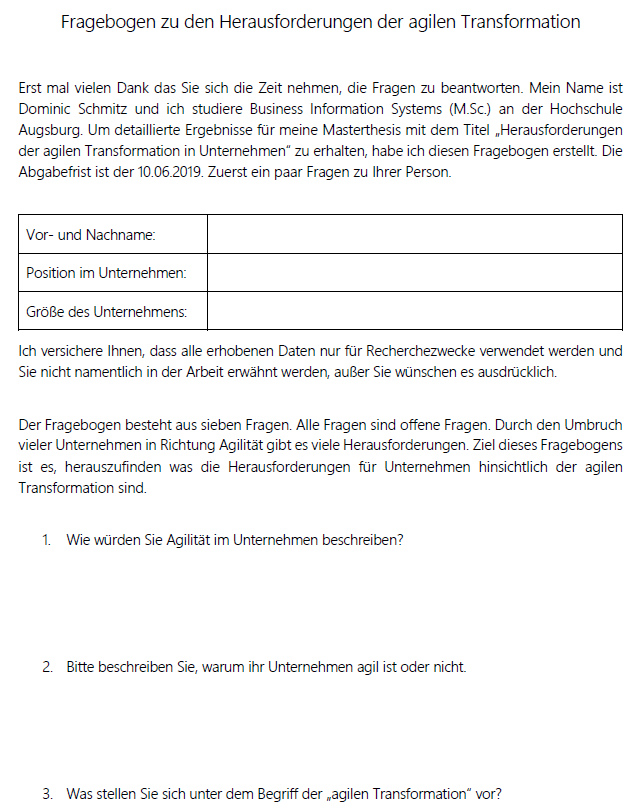
\includegraphics[width=1.0\textwidth]{06_Bilder/Fragebogen_s1.png}
	\setlength{\abovecaptionskip}{1em}
	\caption[]{Fragebogen Seite 1}
	\label{img:anh:fragebogen_s1}
\end{figure}

% Abbildung
\begin{figure}[H]
	\centering
	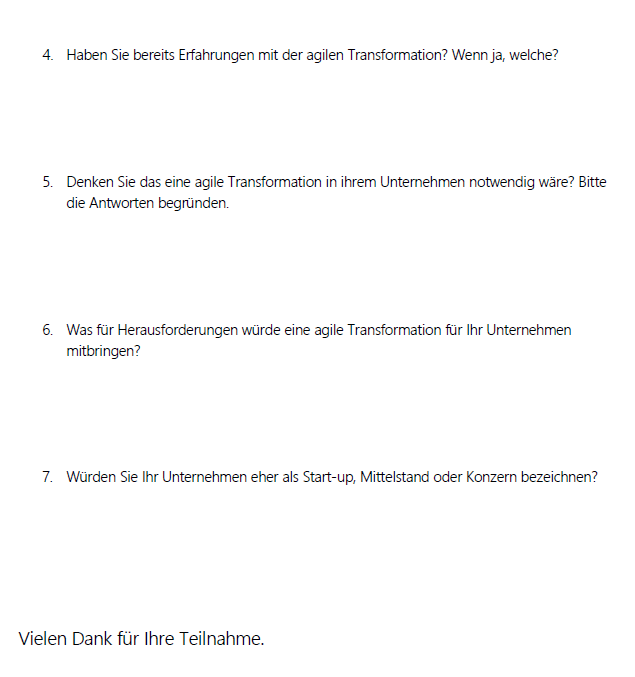
\includegraphics[width=1.0\textwidth]{06_Bilder/Fragebogen_s2.png}
	\setlength{\abovecaptionskip}{1em}
	\caption[]{Fragebogen Seite 2}
	\label{img:anh:fragebogen_s2}
\end{figure}

\phantomsection		
\addstarredchapter{\textbf{Anhang 2, Fragebogen Antworten}} % F�gt "Glossar" zum Inhaltsverzeichnis hinzu	
\chapter*{Anhang 2, Fragebogen Antworten} \label{anh:fragebogen}

\section{Antworten}

\begin{table}[H]
	\centering
	\begin{tabular}{|p{6cm}|p{8cm}|}
		\hline
		\textbf{Position im Unternehmen:}	& Gesch�ftsf�hrer	\\ \hline
		\textbf{Gr��e des Unternehmens:}	& 80 MA 			\\ \hline
	\end{tabular}
	
	\caption{Daten}
	\label{tbl:anh:antw1}
\end{table}

\begin{enumerate}
	\item \textbf{Wie w�rden Sie Agilit�t im Unternehmen beschreiben?}\\
	Agilit�t im Unternehmen bedeutet in erster Linie, dass man als Unternehmen sowie alle Abteilungen und Teams im Einzelnen schnell und unkompliziert auf die sich st�ndig �ndernden �u�eren Faktoren entsprechend reagieren k�nnen. Reagieren hei�t an dieser Stelle nicht \enquote{Dagegenhalten}, sondern diese annehmen und sich m�glichst optimal anpassen oder sogar f�r sich die maximal m�glichen Vorteile daraus ziehen. In agilen Unternehmen h�rt man den Satz \enquote{das haben wir schon immer so gemacht} immer seltener bis gar nicht. Agile Unternehmen sind etwas chaotischer strukturiert, weil nur in einem geordneten Chaos etwas Neues sich formen kann und somit dauerhaft eine Form der Ver�nderung vollzogen wird. 	
	
	\item \textbf{Bitte beschreiben Sie, warum ihr Unternehmen agil ist oder nicht.}\\
	Unser Unternehmen ist agil und soll auch weiterhin agil bleiben. Das Unternehmen geht mit jedem Projekt innovative und zum Teil neue Wege. Mit jedem Projekt, ob es am Ende erfolgreich war oder nicht, gewinnen Mitarbeiter an wertvolle Erfahrung, an neuen Methoden, an neuen Ideen. Es gibt keine feste Teamgrenzen, wir arbeiten vielmehr in virtuellen Teams, die sich auf die Herausforderung jedes Projektes einstellen und neu entstehen. Auch neue Technologien oder neue Methoden werden in unserem Unternehmen nicht nur angenommen, sondern aktiv angewendet und an unsere Kunden weitergegeben. Welche Faktoren sprechen eindeutig daf�r, dass unser Unternehmen agil ist:
	
	\begin{itemize}
		\item Wir haben OKRs eingef�hrt und arbeiten aktiv nach OKR-Modell
		\item Wir haben eine Clean Desk Policy im Unternehmen
		\item Unsere Hierarchien sind sehr flach
		\item Wir sprechen von ?One Team? in dem 80 Mitarbeiter agil arbeiten
		\item Wir erweitern unser Portfolio st�ndig mit neuen Themen
		\item Wir bitten dem Kunden nicht nur das, was wir k�nnen, sondern alles, was wir in der kurzen Zeit vor dem Projektstart noch schaffen zu lernen
		\item Wir haben eine hohe Fehlerkultur, denn nur wer etwas Neues probiert f�llt �fters auf die Nase
		\item Ein GF oder Senior Consultant arbeitet in Projekten auch mit einem Praktikanten zusammen und macht die Sch***-Aufgaben auch alleine 
	\end{itemize}
	
	\item \textbf{Was stellen Sie sich unter dem Begriff der \enquote{agilen Transformation} vor?}\\
	Agile Transformation bedeutet eine dauerhafte Ver�nderung, die sich immer wieder vorsetzt. Eine solche Transformation kann nicht abgeschlossen werden. Sie hat gewisse Etappen, die man erreichen kann, die man auch erreichen muss, aber es geht dann gleich weiter. Es ist eine st�ndige unternehmerische Weiterentwicklung, die gleichzeitig eine Verbesserung ist. Man kann an dieser Stelle sogar von kontinuierlichen Verbesserungsprozessen in einer Organisation sprechen, die zusammengefasst und aus der Flugh�he betrachtet eine agile Transformation des Unternehmens darstellen.
	
	\item \textbf{Haben Sie bereits Erfahrungen mit der agilen Transformation? Wenn ja, welche?}\\
	Fast jeder gr��ere CRM-Ansatz bedeutet eine digitale Transformation, eine neue Art zu arbeiten, mobil zu sein. Solche Projekte werden nicht nur nach agilen Methoden abgearbeitet, sondern legen Grundsteine oder sogar erreichen Etappenziele einer unternehmerischen Transformation. Ob es die gro�e SAFe- oder die kleine SCRUM- Methodik ist, unterscheidet sich die Vorgehensweise im Kern kaum. Mit SAFe wird lediglich die SCRUM-Methodik durch die Skalierung angepasst und sehr breit angewendet. Die Treiber der digitalen Transformation sind in erster Linie die IT-lastige Bereiche eines Unternehmens. F�r die Fachbereiche bedeutet die Transformation gleichzeitig einen Change, daher spielt das Change-Management w�hrend der Transformation eine entscheidende Rolle. Meine Erfahrungen mit der agilen Transformation sind vielseitig, von Neustrukturierung und dadurch Modernisierung der Unternehmensbereiche bis zu IT-Transformation von On-Demand in die Cloud. Dabei arbeiten Gro�konzerne eher nach SAFe-Methodik w�hrend die Mittelst�ndler und Kleinunternehmen von SCRUM sprechen. 
	
	\item \textbf{Denken Sie das eine agile Transformation in ihrem Unternehmen notwendig w�re? Bitte die Antwort begr�nden.}\\
	Ja, diese ist nicht nur notwendig, sondern es ist jedem im Unternehmen Bewusst, dass sich permanent vieles ver�ndern muss, um \enquote{am Ball zu blieben} und dem Mittbewerber immer \enquote{einen Schritt voraus} zu sein. Ob die Ver�nderung in der IT-Landschaft, in der Zusammenarbeit, in der Team-Zusammenstellung oder neue Standorte und neue Themenfelder ? all diese Ver�nderungen geh�ren in unserem Unternehmen zum Alltag und werden von allen Mitarbeitern nicht nur angenommen, sondern auch aktiv mitgestaltet. Wir sind mitten in einer Transformation, mal mehr agil, mal weniger, aber diese Transformation bestimmt unser Arbeitsalltag. Den unsere Kunden erwarten von uns eine Vorbildrolle, was die Digitalisierung angeht, denn wir beraten Sie zu diesen Themen, helfen den Kunden Ihre Herausforderungen in der digitalen Transformation zu schaffen. Denn die Beratungsh�user und Digitale Agenturen sind Pioniere und zugleich die Umsetzer der digitalen Transformation in der Wirtschaft.
	
	\item \textbf{Was f�r Herausforderungen w�rde eine agile Transformation f�r Ihr Unternehmen mitbringen?}\\
	Herausforderungen in folgenden Bereichen:
	\begin{itemize}
		\item \textbf{Interne Organisation:} Durch die stetig wechselnden Projektteams und Themen�berschneidungen ist es schwierig eine interne Organisation so zu fixieren, dass diese zumindest 1-2 Jahre gleich bleibt. Die Herausforderung ist dabei, nach Au�en eine klare Struktur zu zeigen und nach ihnen diese in den Griff zu bekommen ohne klare Grenzen ziehen zu m�ssen.
		
		\item \textbf{Technische Vielfalt:} Die Transformation bring viele technische Tools mit sich, die sinnvoll sind und Mehrwert liefern. Dabei muss man sehr stark aufpassen, dass man sich nicht nur noch mit der Technik besch�ftigt, die einen �berrollt und bereits morgen immer veraltet sein wird egal wie neu diese heute ist. Denn die Transformation bedeutet nicht nur technische Ver�nderung, sondern vielmehr neue Wege gehen, sich immer wieder neu ausrichten, st�ndiges Change Management zu betreiben, neue Methoden auszuprobieren, diese zu Optimieren und neue zu erfinden. Die Technik ist nur Zweck zum Erreichen des Ziels. 
		
		\item \textbf{Den Fokus zu behalten:} Mit st�ndiger Ver�nderung und Neuerung kommt die Gefahr, dass man den Fokus verliert, dass man vergisst, warum man auf dem Markt ist, warum man diese Firma gegr�ndet hat und was man mit der Firma vorhat. Man sollte die gro�en Trends beobachten, sich damit besch�ftigen, aber nicht das gesamte Gesch�ft darauf fokussieren.
		
		\item \textbf{Strategisch zu denken und eine Vision zu haben:} Herausforderung ist dabei, nicht aktionistisch zu handeln, weil es schnell sein muss, sondern strategisch �berlegt. 
		
		\item \textbf{Passende Mitarbeiter zu finden:} Denn nicht jeder mag eine st�ndige Ver�nderung, eine schnelle Entwicklung, Agilit�t in der Arbeit, Vorreiter zu sein. Ein gro�er Teil der in Frage kommenden Mitarbeiter w�rde zwar gerne mitmachen und findet Agilit�t super, aber wenn es dann darauf ankommt, will man 9to5-Job haben und einen festen Arbeitsplatz mit dem Bildrahmen der eigenen Katze auf dem Tisch. Das ist nicht agil, es ist keine Transformation. Das ist SIEMENS-Style bzw. Beamten-Style. 
		
	\end{itemize}
	
	\item \textbf{W�rden Sie Ihr Unternehmen eher als Start-up, Mittelstand oder Konzern bezeichnen?}\\
	Ich w�rde unser Unternehmen noch als Start-up bezeichnen, der auf einem guten Weg zu einem soliden Mittelstand ist. 

\end{enumerate}

\newpage

\section{Antworten}

\begin{table}[H]
	\centering
	\begin{tabular}{|p{6cm}|p{8cm}|}
		\hline
		\textbf{Position im Unternehmen:}	& Spezialist Test Management	\\ \hline
		\textbf{Gr��e des Unternehmens:}	& 200 MA 			\\ \hline
	\end{tabular}
	
	\caption{Daten}
	\label{tbl:anh:antw2}
\end{table}

\begin{enumerate}
	\item \textbf{Wie w�rden Sie Agilit�t im Unternehmen beschreiben?}\\
	Agilit�t bedeutet Verantwortung f�r das eigene Handeln zu �bernehmen sowie Freir�ume und Flexibilit�t f�r die L�sung von Problemstellungen so zu nutzen, dass das bestm�gliche Ergebnis f�r das Unternehmen entsteht.	
	
	\item \textbf{Bitte beschreiben Sie, warum ihr Unternehmen agil ist oder nicht.}\\ 
	Mein Unternehmen ist intern bereits sehr agil, da flache Hierarchien bestehen. Au�erdem sind Teams vorhanden, die nach Scrum und Kanban arbeiten sowie Konfliktmanagementprozesse, die es auf verschiedenen Stufen erm�glichen, Konflikte mit neutralen Kollegen in 1:1 Gespr�chen oder im Team zu l�sen. Dar�ber hinaus kann sich jeder einzelne Kollege einbringen und wird auch geh�rt. In der Zusammenarbeit mit externen Partnern sind wir weniger agil unterwegs, da viele externe Kollegen sehr an Hierarchien glauben und nicht selber Verantwortung f�r das eigene Handeln �bernehmen wollen. Hier ist noch die Denke vertreten: \enquote{Ich mache das, was man mir sagt, dann bekomme ich mein Geld}. Wir versuchen die Leute nun nach und nach weiter zu entwickeln, um auch da wirklich agil zu werde.
	
	\item \textbf{Was stellen Sie sich unter dem Begriff der \enquote{agilen Transformation} vor?}\\
	Agile Transformation ist f�r mich der Weg von einem hierarchischen Betriebsmodell hin zu einem agilen Unternehmen. Dieser Weg ist f�r jedes Unternehmen individuell und muss entsprechend geplant werden, damit alle Mitarbeiter abgeholt werden k�nnen.
	
	\item \textbf{Haben Sie bereits Erfahrungen mit der agilen Transformation? Wenn ja, welche?}\\
	Ja, habe ich. In verschiedenen Unternehmen war ich bei der Planung von Workshops beteiligt oder habe als QA, PO und Scrum Master agile Teams mit aufgebaut. Die Transformationen waren nicht immer leicht, da es besonders darauf ankommt Kollegen zu haben, die offen f�r die Transformation sind. Verschlie�t sich jemand, ist es oftmals unm�glich die Leute zu �berzeugen und sie verlassen �ber kurz oder lang das Unternehmen.
	
	\newpage
	\item \textbf{Denken Sie das eine agile Transformation in ihrem Unternehmen notwendig w�re? Bitte die Antwort begr�nden.}\\
	Die Transformation ist bei uns in Gange und wird auch nie abgeschlossen sein, da man sich immer weiterentwickeln und verbessern kann.
	
	\item \textbf{Was f�r Herausforderungen w�rde eine agile Transformation f�r Ihr Unternehmen mitbringen?}\\
	\begin{itemize}
		\item Externe Mitarbeiter mit eingliedern 
		\item Gegner �berzeugen
		\item Mitarbeiter enabeln Verantwortung zu �bernehmen 
		\item Zusammenarbeit mit dem Mutterkonzern, der noch sehr nach Wasserfall-lastig arbeitet
	\end{itemize}
	
	\item \textbf{W�rden Sie Ihr Unternehmen eher als Start-up, Mittelstand oder Konzern bezeichnen?}\\
	Wir sind der agile Part eines Konzerns
	
\end{enumerate}

\newpage

\section{Antworten}

\begin{table}[H]
	\centering
	\begin{tabular}{|p{6cm}|p{8cm}|}
		\hline
		\textbf{Position im Unternehmen:}	& 	VP Product Strategy\\ \hline
		\textbf{Gr��e des Unternehmens:}	& 	50 MA		\\ \hline
	\end{tabular}
	
	\caption{Daten}
	\label{tbl:anh:antw3}
\end{table}

\begin{enumerate}
	\item \textbf{Wie w�rden Sie Agilit�t im Unternehmen beschreiben?}\\
	\enquote{Agile} geht Hand in Hand mit anderen Konzepten wie \enquote{Lean} und \enquote{Management 3.0}. In meinen Augen ist es vor allem ein Wertesystem und ein Werkzeugkasten. Die Werte sind den Anforderungen einer modernen, digitalen Arbeits- und Gesch�ftswelt angepasst. Aus dem Werkzeugkasten kann man sich bedienen um eine f�r das eigene Unternehmen passenden L�sung zu schaffen. Agilit�t besteht nicht nur aus Prozessen und Workflows, die man kopieren/lernen kann.
	\\\\
	Agilit�t bottom-up einzuf�hren funktioniert aus meiner Erfahrung nicht ? top-down aber auch nicht, wenn das Executive-Management glaubt, dass das ohne Ver�nderungen f�r sie selber m�glich ist oder nicht an die zugrunde liegenden Werte  und Benefits glaubt.
	\\\\
	Es gibt kein Blueprint, es gibt nicht sowas wie \enquote{das Spotify-Modell}. Man kann \enquote{Agilit�t} einem Unternehmen nicht \enquote{verordnen}, durch Consultants beibringen. Man committet sich auf die Werte ? durch alle Managementlevel - und kann sich Unterst�tzung holen den Werkzeugkasten richtig einzusetzen.
	\\\\
	Der Gedanke vom \enquote{lernenden Unternehmen}, das sich permanent weiterentwickelt und der Ver�nderungen anpasst, wird sehr oft au�en vor gelassen/vergessen.
	\\\\
	Agilit�t betrifft alle Aspekte eines Unternehmens ? von der Organisationsstruktur bis zum Zielsystem. Sie ist nichts, was nur \enquote{in der Technik} oder ausschlie�lich in Entwicklungsteams stattfindet. Transformationen, die nur eine Abteilung im Unternehmen betreffen, scheitern schnell.
	\\\\
	Agilit�t wird auch gerne mit \enquote{chaotisch} oder \enquote{ich darf doch als Manager jeden Tag meine Meinung �ndern, oder?} verwechselt.
	\\\\
	Ein sehr h�ufiges Problem ist auch der verbliebene Wunsch nach langfristiger Milestone-Planung, der mit Agilit�t nicht vereinbar ist bzw. den die Agile Welt als nicht sinnvoll darstellt.
		
	
	\item \textbf{Bitte beschreiben Sie, warum ihr Unternehmen agil ist oder nicht.}\\
	Die Bandbreite ist hoch: einzelne Teams arbeiten agiler als andere. Einige Elemente aus dem agilen Werkzeugkasten sind umgesetzt ? aber viele auch nicht. Agile wird nicht durch das gesamte Unternehmen und alle Hierarchieebenen gelebt. Die dem \enquote{Agile} Gedanken zugrundeliegende Werte und Benefits werden aber auch nicht vollst�ndig als valide gesehen.
	\\\\
	Bei Einzelpersonen gibt es auch eine gewisse \enquote{Agile M�digkeit}: Ver�nderungsversuche aus der Vergangenheit, die nicht erfolgreich waren (aus unterschiedlichen Gr�nden), werden der Grundidee angelastet ? dadurch wird zu Weile eher polemisch �ber \enquote{Agile} gesprochen, vor allem im Senior/Executive Management (die klassischer Weise den meisten \enquote{Machtverlust} erleiden, wenn man ein Unternehmen voll und ganz Agile f�hren will).
	\\\\
	Insgesamt ist die Agilit�t f�r ein konzern-nahes Unternehmen vermutlich gar nicht so schlecht, aber gemessen an Digital Champions oder Start-ups sehr bescheiden. Das liegt IMHO vor allem daran, dass das Management nicht an die Ideen und Werte glaubt ? oder nicht bereit ist in die Transformation zu investieren bzw. den damit verbundenen Machtverlust zu akzeptieren.
	
	\item \textbf{Was stellen Sie sich unter dem Begriff der \enquote{agilen Transformation} vor?}\\
	Ich mag den Begriff nicht sehr. F�r mich schwingt da mit, dass man die Mitarbeiter umformt und sie dann nach Projektabschluss am Ziel sind.
	\\\\
	Die Werkzeuge der Agile Community entwickeln sind permanent weiter.
	Ohne mich zu sehr wiederholen zu wollen: man sollte sich auf die Werte committen und die Weichen stellen ein lernendes Unternehmen zu werden ? dann kann man eigentlich dauerhaft die notwendigen Ver�nderungen vornehmen, ohne das man jemals komplett am Ziel ist. Ver�nderung als Dauerzustand.
	
	\item \textbf{Haben Sie bereits Erfahrungen mit der agilen Transformation? Wenn ja, welche?}\\
	Ja, viele. Von Ans�tzen auf der Teamebene, der Abteilungsebene (beides bottom-up), bis zur unternehmensweiten Mission. Wenige allerdings mit nachhaltigen und guten Erfolgen. Zumeist ist es an den Dingen gescheitert, die ich bereits in den vorherigen Antwortet erw�hnt habe.
	\\\\
	Zwischenzeitlich war ich sogar hauptverantwortlich (\enquote{Chief Agile Coach}) f�r die agile Unternehmenskultur und Ver�nderung. Obwohl ich sehr leidenschaftlich an manche der agilen Ideen glaube, habe ich diese Aufgabe am Ende abgegeben ? weil es einfach zu frustierend war in der Umsetzung. Ich habe mir auch vorgenommen ? obwohl ich in dem Bereich einige Erfahrung habe ? nur dann noch mal in einer �hnlichen Rolle in einem anderen Unternehmen t�tig zu werden, wenn ich 100\% davon �berzeugt bin, dass die Unternehmensf�hrung die Konzepte versteht und hinter den Werten steht.
	
	\item \textbf{Denken Sie das eine agile Transformation in ihrem Unternehmen notwendig w�re? Bitte die Antwort begr�nden.}\\
	Ja, ich glaube nach wie vor daran, dass das Unternehmen von mehr \enquote{richtiger} Agilit�t profitieren w�rde: bessere Zusammenarbeit �ber alle Abteilungen, mehr Transparenz; mehr F�higkeit schnell auf den Markt zu reagieren; Ideen schneller austesten und verwerfen, wenn sie nicht genug Potential beweisen, ...
	
	\item \textbf{Was f�r Herausforderungen w�rde eine agile Transformation f�r Ihr Unternehmen mitbringen?}\\
	\begin{itemize}
		\item Nachdem wir in einen Konzern eingebettet sind: Strukturen au�erhalb des Unternehmens, an den Schnittpunkten zum (nicht-agilen) Konzern kompatible zur eigenen Agilit�t machen
		\item Lehre und �berzeugungsarbeit im Senior-Management (Machtverlust kompensieren/akzeptieren)
		\item Wir sitzen an zwei Standorten, bei dem einer auch noch in einem anderen Kulturkreis ist (Ukraine); alle Mitarbeiter mitzunehmen, die agilen Werte zu vermitteln, ist eine nicht zu untersch�tzende Herausforderung
		\item Das Investment der Transformation und die damit verbundenen kurzfristigen Abstriche in der Produktivit�t zu Gunsten der mittel- bis langfristigen Vorteile akzeptieren
	\end{itemize}
	
	\item \textbf{W�rden Sie Ihr Unternehmen eher als Start-up, Mittelstand oder Konzern bezeichnen?}\\
	Hybrid: Start-up like (�hnliche Herausforderungen, partiell Autonomie eines Start-ups), aber eng eingebettet in einen Konzern; Mitarbeiter-Struktur, HR-Themen sind sehr Konzern-nah.
	
\end{enumerate}

\newpage

\section{Antworten}

\begin{table}[H]
	\centering
	\begin{tabular}{|p{6cm}|p{8cm}|}
		\hline
		\textbf{Position im Unternehmen:}	& 	\\ \hline
		\textbf{Gr��e des Unternehmens:}	& 			\\ \hline
	\end{tabular}
	
	\caption{Daten}
	\label{tbl:anh:antw4}
\end{table}

\begin{enumerate}
	\item \textbf{Wie w�rden Sie Agilit�t im Unternehmen beschreiben?}\\	
	
	\item \textbf{Bitte beschreiben Sie, warum ihr Unternehmen agil ist oder nicht.}\\ 
	
	\item \textbf{Was stellen Sie sich unter dem Begriff der \enquote{agilen Transformation} vor?}\\
	
	\item \textbf{Haben Sie bereits Erfahrungen mit der agilen Transformation? Wenn ja, welche?}\\
	
	\item \textbf{Denken Sie das eine agile Transformation in ihrem Unternehmen notwendig w�re? Bitte die Antwort begr�nden.}\\
	
	\item \textbf{Was f�r Herausforderungen w�rde eine agile Transformation f�r Ihr Unternehmen mitbringen?}\\
	
	\item \textbf{W�rden Sie Ihr Unternehmen eher als Start-up, Mittelstand oder Konzern bezeichnen?}\\
	
\end{enumerate}

\newpage

\section{Antworten}

\begin{table}[H]
	\centering
	\begin{tabular}{|p{6cm}|p{8cm}|}
		\hline
		\textbf{Position im Unternehmen:}	& 	\\ \hline
		\textbf{Gr��e des Unternehmens:}	& 			\\ \hline
	\end{tabular}
	
	\caption{Daten}
	\label{tbl:anh:antw5}
\end{table}

\begin{enumerate}
	\item \textbf{Wie w�rden Sie Agilit�t im Unternehmen beschreiben?}\\	
	
	\item \textbf{Bitte beschreiben Sie, warum ihr Unternehmen agil ist oder nicht.}\\ 
	
	\item \textbf{Was stellen Sie sich unter dem Begriff der \enquote{agilen Transformation} vor?}\\
	
	\item \textbf{Haben Sie bereits Erfahrungen mit der agilen Transformation? Wenn ja, welche?}\\
	
	\item \textbf{Denken Sie das eine agile Transformation in ihrem Unternehmen notwendig w�re? Bitte die Antwort begr�nden.}\\
	
	\item \textbf{Was f�r Herausforderungen w�rde eine agile Transformation f�r Ihr Unternehmen mitbringen?}\\
	
	\item \textbf{W�rden Sie Ihr Unternehmen eher als Start-up, Mittelstand oder Konzern bezeichnen?}\\
	
\end{enumerate}

\chapter*{Anhang 3, Interviews}

\textbf{Anmerkung: } Die hier aufgef�hrten Interviews wurden am 06.06.2019 gef�hrt. Die Befragung wurde von Herrn Dominic Schmitz (Autor dieser Arbeit) gef�hrt. Die komplette Befragung wird als .mp3 Datei, dieser Arbeit zugegeben. Folgend wird das gesprochene Wort in Text umgewandelt. Hierbei ist wichtig zu erw�hnen, dass grammatikalische Fehler im besten gewissen verbessert wurden. Dabei wird in keiner wei�e die Bedeutung des Satzes und dessen Informationen ver�ndert. Die hierbei verwendeten Fragen, beziehen sich grundlegend auf die, des Fragebogens aus Anhang \ref{anh:fragebogen}. Es kommt vor, dass zus�tzliche Fragen bez�glich einer Antwort gestellt wurden.

\section{Interview Caroline Wicks Schmitz}

\begin{table}[H]
	\centering
	\begin{tabular}{|p{6cm}|p{8cm}|}
		\hline
		\textbf{Vorname, Nachname:} 		& 	Caroline, Wicks Schmitz			\\ \hline
		\textbf{Position im Unternehmen:}	& 	Chief Financial Officer (CFO)	\\ \hline
		\textbf{Name des Unternehmens:} 	&	C. \& E. Fein GmbH				\\ \hline 
		\textbf{Gr��e des Unternehmens:}	&	ca. 950 MA / 750 Mio. Umsatz im Jahr\\ \hline
	\end{tabular}
	
	\caption{Daten}
	\label{tbl:anh:int1}
\end{table}

\begin{itemize}
	\item \textbf{Wie lautet ihr vollst�ndiger Name?}\\
	Ich hei�e Caroline Wicks Schmitz. Ich bin derzeit CFO (Chief Financial Officer) der Fein Gruppe. Das ist ein Unternehmen mit weltweit circa 950 Mitarbeiternc und einem Jahresumsatz von circa 170 Millionen Euro. 
	
	\item \textbf{Sie willigen ein, dass die Befragung und die hier erhobenen Daten f�r diese Masterthesis verwendet werden d�rfen?}\\
	Selbstverst�ndlich willige ich ein.
	
	\item \textbf{Wie w�rden Sie Agilit�t im Unternehmen beschreiben?}\\
	Grunds�tzlich ist Agilit�t f�r mich eine Methode der Projektverfolgung, die Bewegung und Innovation im Unternehmen f�rdert, im Gegensatz zum klassischen Projektmanagement, dass eher einen starren Ablauf vordefiniert. Bei Fein w�rde ich sagen, dass eher das klassische Projektmanagement verwendet wird. Es werden Meilensteine definiert die den Zielen der Sprints aus agilen Formen �hneln. Zus�tzlich wird auch eine Zielplanung durchgef�hrt und es gibt review Meetings, die nicht t�glich abgehalten werden, sondern im klassischen Sinne nach erreichen eines Meilensteins. F�r die Firma Fein sind die Produktentwicklungsprojekte sehr wichtig im Projektmanagement. Dort gibt es wirklich diesen klassisch definierten Ablauf, wie ein Produkt definiert wird. Ich denke das vielleicht eine agile Vorgehensweise in diesem Bereich mehr Innovation und Kreativit�t fordern k�nnte.
	
	\item \textbf{Sie w�rden also ihren momentanen Prozess als Iterativ bezeichnen, aber die agilen Methodiken w�ren dann doch zukunftstr�chtiger?}
	Ich denke schon, dass da etwas zu gewinnen w�re. In einer klassischen Projektentwicklungsform, gehen die Ingenieure nur Schritt f�r Schritt vor hacken ihre Listen ab. In diesem Bereich w�rde nat�rlich diese reaktive Form der Agilit�t helfen selbst�ndiges Mitdenken, Kreativit�t und Eigeninitiative zu f�rdern.
	
	\item \textbf{Bitte beschreiben Sie, warum ihr Unternehmen agil ist oder nicht.}\\ 
	Ich w�rde Fein nicht als agil beschreiben, weil man eher von oben herab dieses Management by Command and Control hat. Dadurch haben die Mitarbeiter nicht den Mut Entscheidungen selber zu treffen. Das hat zur Folge, dass die Entscheidungsfreiheit und Motivation verloren geht. Die Mitarbeiter haben auch Angst vor offenen Feedback. Oft wird der Hinweis auf Fehler noch missverstanden, da die Mitarbeiter in der Unternehmenskultur noch nicht in der Lage sind, die Vorteile von offenem Feedback zu erkennen. Zus�tzlich wirkt das normale Tagesgesch�ft dagegen. Ich denke jeder Mitarbeiter hat einen hohen Anteil an Tagesgesch�ft und die Bereichs�bergreifende Zusammenarbeit wird dadurch nicht erleichtert.
	
	\item \textbf{Was stellen Sie sich unter dem Begriff der \enquote{agilen Transformation} vor?}\\
	Also f�r mich muss erst eine Basis zur agilen Transformation vorhanden sein. Es muss die Unternehmenskultur stimmen und von ganz oben herab eine Kultur der Offenheit und des Vertrauens gefordert werden. Wenn gen�gend Kapazit�ten frei sind, m�ssten von oben herab diese agilen Werte und Prinzipien zuerst gelehrt und ge�bt werden. Hierf�r m�ssten vielleicht anfangs ein paar kleinere Projekte die nicht Bereichs�bergreifend sind abgewickelt werden. So k�nnen Mitarbeiter diese Werte und Prinzipien erst mal �ben und lernen. Wichtig dabei ist, klar die Vision des Unternehmens, also wohin will das Unternehmen und was bringt uns das ganze, zu vermitteln. 
	
	\item \textbf{W�rden Sie die agile Transformation als Prozess der abgeschlossen werden kann sehen?}\\
	Nein, ich glaube das ist immer etwas das ge�bt werden muss. Nat�rlich werden manche Mitarbeiter mehr �bung als andere haben. Zus�tzlich wird es immer neue Mitarbeiter und andere Projekte mit anderen Zielen geben. Aus diesem Grund ist f�r mich die agile Transformation ein Prozess der nicht einfach so abgeschlossen werden kann. Irgendwann wird es ins Blut �bergehen, aber das ist ein Prozess der l�nger dauern wird. 
	
	\item \textbf{Haben Sie bereits Erfahrungen mit der agilen Transformation? Wenn ja, welche?}\\
	Bei Fein wurde noch keine agile Transformation durchgef�hrt, aber es wurden bereits �hnliche Elemente eingesetzt. Verwendet hatten wir KVP, also kontinuierliche Verbesserungsprozesse, bei denen wir uns immer weiter verbessert hatten. Dieser Prozess war auch nie abgeschlossen, sondern man setzt sich immer mit der Gruppe zusammen und verbessert kontinuierlich. Das wurde allerdings von der neuen Gesch�ftsf�hrung abgeschafft, weshalb ich sagen w�rde, dass Fein nicht agil Arbeitet und auch keine ansinnen danach besitzt.
	
	\item \textbf{Also will Fein zuk�nftig nicht agil agieren?}\\
	Ich hatte es schon einmal hochgebracht, aber da habe ich einfach nur gro�e Fragezeichen bei den Leuten und der Gesch�ftsf�hrung gesehen. 
	
	\item \textbf{Denken Sie das eine agile Transformation in ihrem Unternehmen notwendig w�re? Bitte die Antwort begr�nden.}\\
	Fein ist ein Traditionsunternehmen und besitzt �ber 150 Jahre Geschichte. Wir entwickeln und produzieren Elektrowerkzeuge und besitzen eine Entwicklung mit etwa 70 bis 80 Mitarbeitern. Ich denken auf jeden Fall im Entwicklungsbereich w�re die Beweglichkeit und der permanente Wandel, die Motivation und die Kreativit�t die ein agiles Vorgehen schaffen w�rde, sehr Hilfreich innovative neue Produkte zu entwickeln. Leider sind die Voraussetzungen, die durch eine entsprechende Unternehmenskultur geschaffen werden, noch nicht vorhanden. Diese m�ssten agile Vorgehensweisen unterst�tzten bevor man anf�ngt so zu arbeiten.
	
	\item \textbf{Was f�r Herausforderungen w�rde eine agile Transformation f�r Ihr Unternehmen mitbringen?}\\
	Herausforderungen w�ren das schon viele. Als erstes muss eine entsprechende Unternehmenskultur geschaffen werden, die eine entsprechende Vorgehensweise f�rdert. Ein gro�es Thema bez�glich dessen, ist die bereichs�bergreifende Zusammenarbeit bei der ich viele Herausforderungen sehe. Ein Beispiel ist das Daily Scrum. Es w�re so gut wie unm�glich im klassischen Weg, w�hrend eines Projektablaufs, allein schon einmal pro Woche Leute zusammen zu rufen, sich eine habe Stunde zusammen zu setzen. Das ist deshalb so schwierig, da jeder Bereich seine eigenen Projekte und sein eigenes Tagesgesch�ft besitzt. Hier die notwendigen Mitarbeiter regelm��ig zusammen zu bekommen ist schon ein Problem. Wenn ich allerdings sehe, was w�chentlich alles passiert, wie viele Informationen dort weitergegeben werden und wie das Team dann zusammenwachsen w�rde, w�re das schon sehr interessant t�glich ein Meeting zu veranstalten. Aber bei uns hat die Entwicklung manchmal um die 100 Projekte gleichzeitig am laufen, wie sollen die dann 100 Daily Scrums am Tag abhalten? Das mal abgesehen von irgendwelchen Projekten, die die IT oder irgend welche anderen Abteilungen im Unternehmen gerade durchf�hren. 
	
	\item \textbf{Also gibt nur Herausforderungen hinsichtlich der Meetings und der Kultur?}\\
	Grunds�tzlich sehe ich die Herausforderungen in der Unternehmenskultur, da diese sehr traditionell Deutsch ist. Fehler werden eher verp�hnt, als das diese als Opportunity gesehen werden, irgendwas zu verbessern. Zus�tzlich m�ssten Mitarbeiter mehr Vertrauen bekommen, dass es auch OK ist Fehler zu machen. Das was hierbei gelernt wird, w�rde die Firma auch weiter bringen. Das ist aber auch noch nicht vorhanden. Ein weiterer Punkt ist der, dass viele Prozesse einfach schon festgelegt sind und der Gedanke \enquote{bis jetzt hat es immer so geklappt, warum sollten wir daran etwas �ndern} noch vorhanden ist. In Wirklichkeit klappt eigentlich nichts, da wir mit dem traditionellen Gedanken nicht die notwendigen neuen innovativen Produkte entwickeln k�nnen. 
	
	\item \textbf{W�rden Sie Ihr Unternehmen eher als Start-up, Mittelstand oder Konzern bezeichnen?}\\
	Von den Statistiken her, sind wir wahrscheinlich ein Konzern. Das liegt an der H�he des Umsatzes und der Anzahl der Mitarbeiter. Das Denken im Unternehmen, entspricht eher dem des Mittelstands. Fein ist ein familiengef�hrtes traditionelles Unternehmen. Aus diesem Grund w�rde ich es eher als eine Kombination aus beiden beschreiben. 
	
	\item \textbf{W�rden Sie behaupten das die agile Transformation dem Mittelstand schwerer f�llt als anderen Unternehmensformen?}\\
	Ich denke schon, dass die agile Transformation dem Mittelstand schwerer f�llt, da der Mittelstand hier in Deutschland, traditionell sehr erfolgreich ist. Der deutsche Mittelstand ist der Wirtschaftsmotor Deutschlands. Diese Form von Unternehmen sind h�ufig Familiengef�hrte Unternehmen, die viel Erfolg �ber die Jahre und auch gute Ergebnisse gezeigt haben. Zus�tzlich wird dieses Management by Command and Control praktiziert und die Denkweise spiegelt bis jetzt sehr stark den Gedanken: \enquote{bis jetzt hat es immer so geklappt, warum sollten wir daran etwas �ndern}. Ver�nderung bei vielen mittelst�ndischen Firmen ist schwierig. Viele Merken das es Vorteile Bringt aber es liegt einfach noch nicht in deren Genen und Blut sich auf jede neue Ver�nderung zu st�rzen. H�ufig sind sie eher passiv, warten ab und schauen was andere machen bevor sie sich selbst ver�ndern. 
	
	\item \textbf{Also w�rden Sie eher den Wandel als langsam beschreiben?}\\
	Ja, sehr konservativ, sehr vorsichtig, erst mal schauen was passiert und ob es sich hierbei um eine Modeerscheinung handelt? Wieso sollen wir Geld investieren, wenn unsere klassische Denkweise uns auch voran gebracht hat?
	
	\item \textbf{Denken Sie das Konzerne einen schnelleren Wandel durchlaufen?}\\
	Konzerne werden mehr mit neuen Methodiken konfrontiert als der Mittelstand. Sie besitzen auch mehr Kapazit�ten und besitzen vielleicht auch mehr Stakeholder und Projectowners die Interesse an einer neuen Methode h�tten und so einen Wandel voran treiben. 
\end{itemize}


\section{Interview Otto-Max Herbstritt}

\begin{table}[H]
	\centering
	\begin{tabular}{|p{6cm}|p{8cm}|}
		\hline
		\textbf{Vorname, Nachname:} 		& 	Otto-Max Herbstritt				\\ \hline
		\textbf{Position im Unternehmen:}	& 	Chief Information Officer (CIO)	\\ \hline
		\textbf{Name des Unternehmens:} 	&	C. \& E. Fein GmbH				\\ \hline 
		\textbf{Gr��e des Unternehmens:}	&	ca. 950 MA	 					\\ \hline
	\end{tabular}
	
	\caption{Daten}
	\label{tbl:anh:int2}
\end{table}

\begin{itemize}
	\item \textbf{Wie lautet ihr vollst�ndiger Name?}\\
	Otto-Max Herbstritt.
	
	\item \textbf{Wie lautet ihre aktuelle Position?}\\
	Ich bin selbst�ndig als Interims CIO.
	
	\item \textbf{Was f�r eine Position haben sie bei Fein ausge�bt?}\\
	C. \& E. Fein GmbH, Chief Information Officer (CIO).
	
	\item \textbf{Sie willigen ein das die erhobenen Daten der Befragung f�r diese Masterarbeit verwendet werden d�rfen?}\\
	Ja.
	
	\item \textbf{Wie w�rden Sie Agilit�t im Unternehmen beschreiben?}\\
	Ich kann diese Frage nur auf IT-Projekte beziehen. Bei Fein gab es erst einmal keine Agilit�t. Wir hatten ein agiles Projekt mit dem Thema der CRM Einf�hrung aber das lief aus meiner Sicht genauso wie ein normales Projekt. Die IT-Projekte wurden von mir immer bei Fein vorangetrieben, dort habe ich pers�nlich agil gehandelt. Es gab w�chentliche Meetings mit den Projektteilnehmern und Mitarbeitern und ich hab mich, sofern es notwendig war, immer mit dem Fachbereich abgestimmt. Wenn ich ein agiles Projekt im Unternehmen Fein beschreiben m�sste, kann ich das nicht, denn es gab keins. Ich pers�nlich w�rde iterativ vorgehen wenn ich agil handeln w�rde. Das was man fr�her in einem St�ck erledigt hat, wird jetzt in mehreren St�cken erledigt.
	
	\item \textbf{Bitte beschreiben Sie, warum ihr Unternehmen agil ist oder nicht.}\\
	Wie schon erw�hnt, Fein geht in der IT nicht agil vor, da die Projektzeiten eigentlich immer festgelegt wurden auf ein Jahr und in diesem Zeitraum auch abgeschlossen wurden. Im Rahmen dieses Zeitfensters gab es auch nur einen Abschluss. Zus�tzlich gab es immer gen�gend Zeit die Projekte vern�nftig zu planen mit entsprechender Luft. Des Weiteren war es auch so, dass ich gar keine Chance f�r das agilen Projektmanagement gesehen habe. Es wurden die Mitarbeiter ausgebildet, aber nicht f�r agile Herangehensweisen. Wenn dies doch der Fall ist, m�ssen alle mitmachen, nicht nur die IT-Abteilung. Aus diesen Gr�nden w�rde ich unser Unternehmen nicht als agil bezeichnen. 
	
	\item \textbf{Was stellen Sie sich unter dem Begriff der \enquote{agilen Transformation} vor?}\\
	Darunter stelle ich mir vor, dass die ganze Firma, alle Projekte agil steuert. Beispielsweise mithilfe eines Frameworks wie etwa Scrum. Um dies allerdings zu verwirklichen m�ssen alle Mitarbeiter hinreichend geschult werden. Jeder Mitarbeiter im Unternehmen muss diese Vorgehensweise auch unterst�tzten damit dies Erfolg bringt. Wenn es nicht unterst�tzt wird, und beispielsweise ein Mitarbeiter Schwierigkeiten macht, tauchen die ersten Probleme auf. Somit muss die ganze Firma darauf ausgerichtet sein, alle Mitarbeiter entsprechend geschult werden und in der Lage sein sich daf�r Zeit zu nehmen. Diese Zeit ist in vielen Unternehmen gar nicht gegeben, da das Gesamtheitliche nicht gesehen wird und jeder Mitarbeiter sein eigenes Tagesgesch�ft besitzt. Auch die Bereichs�bergreifenden Prozesse m�ssen angepasst werden und Vorgesetzte m�ssen entsprechende Konsequenzen tragen. Oft denken allerdings die Fachbereiche nicht Bereichs�bergreifend was zus�tzlich zu Problemen f�hrt. 
	
	\item \textbf{Haben Sie bereits Erfahrungen mit der agilen Transformation? Wenn ja, welche?}\\
	Nein.
	
	\item \textbf{Denken Sie das eine agile Transformation in ihrem Unternehmen notwendig w�re? Bitte die Antwort begr�nden.}\\
	Ja, ist notwendig, da Gesch�ftsprozesse oft Bereichs�bergreifend sind. Wenn nur die IT die Projekte vorantreibt und die Fachbereiche den Gedanken \enquote{Ist ja nur ein IT-Projekt} besitzen, funktioniert das nicht. Auch die Fachbereiche m�ssen mithelfen und die Kapazit�ten zur Verf�gung stellen und die Zeit daf�r aufbringen (gegeben falls Freistellen), damit gerade agile Prozesse umgesetzt werden k�nnen. Ich wei� die Frage bezieht sich auf die Transformation, allerdings w�re es schon mal sch�n einen Vergleich zwischen einem nicht agilen und agilen Projekt zu sehen.
	
	\item \textbf{Was f�r Herausforderungen w�rde eine agile Transformation f�r Ihr Unternehmen mitbringen?}\\
	Erstmal muss die Zusammenarbeit von oben nach unten verbessert werden. Das bedeutet, dass auch die Gesch�ftsf�hrung dahinter stehen muss. Sie sollte nicht nur \enquote{Br�llen} wenn etwas nicht funktioniert. 
	Vorgesetzte m�ssen akzeptieren das Mitarbeiter mehr Zeit ben�tigen. So muss das Verst�ndnis aufgebracht werden, dass weniger Zeit f�r das Tagesgesch�ft vorhanden ist, da die Aufgaben des Sprints auch erledigt werden m�ssen. Alle Mitarbeiter m�ssen auch geschult werden hinsichtlich des agilen Projektmanagements, damit sie erfahren f�r was das alles gut ist. Zus�tzlich sollte noch eine Stelle geschaffen werden, die entsprechende KPI�s hat um das zentrale Projektmanagement auch entsprechend zu managen. Diese Stelle sollte in der Lage sein zu sagen, da haben wir ein Problem, da muss gehandelt werden. Das sollte relativ neutral passieren, damit der entsprechende Business Owner in dem es das Problem gibt auch reagieren kann. 
	
	\item \textbf{W�rden Sie Ihr Unternehmen eher als Start-up, Mittelstand oder Konzern bezeichnen?}\\
	Fein ist Mittelstand. 
	
	\item \textbf{W�rden Sie behaupten das die agile Transformation dem Mittelstand schwerer f�llt als anderen Unternehmensformen?}\\
	Es kommt auf die F�hrungskultur an und wie gro� der Mittelstand ist. Wenn ich einen kleinen Mittelstand nehme, zwischen 50 und 100 Mitarbeitern f�llt es denen sicherlich schwer, weil die nicht laufend so viele Projekte machen und alle sehr Hands-on sind, da sie sonst nicht Flexibel w�ren. Der gro�e Mittelstand wie beispielsweise Fein, k�nnte es durchaus umsetzen, wenn konsequent die Gesch�ftsf�hrung auch dahinter w�re und die Mitarbeiter machen l�sst, ohne dauernd rein zu funken, wenn denen etwas nicht gef�llt. Zusammengefasst w�rde ich also behaupten das es dem kleinen Mittelstand schwerer f�llt, hingegen dem gro�en einfacher. Das liegt daran das der kleine Mittelstand pragmatischer Orientiert ist als der gro�e.
	Zus�tzlich h�ngt es nat�rlich auch von den Projekten ab und wie diese definiert sind. Wenn ein Projekt durchgef�hrt wird, sieht man es aus Unternehmenssicht strategisch, da ein Ziel erreicht werden soll. Aus Anwendersicht wird es nicht strategisch gesehen, denn dieser will einfach nur schnell sein Problem gel�st haben. Die Anwendersicht wird h�ufig im kleinen Mittelstand vertreten hingegen beim gro�en Mittelstand eher die strategische. 
	Ein weiterer Aspekt ist die Abh�ngigkeit der verschiedenen Systeme und wie diese miteinander verkn�pft sind. Fein besitzt sehr viele Systeme und automatisierte Prozesse im Vergleich zu anderen Unternehmen, was nat�rlich eine Transformation noch einmal zus�tzlich erschwert. 
	
	
\end{itemize}




%-----------------------------------------------------------------------------
% END OF DOCUMENT														  ---------------------
%-----------------------------------------------------------------------------
\end{document}

